\section{Kết quả thực nghiệm và biểu đồ}

Lưu ý: Hai thuật toán Bubble Sort, Shaker Sort trong thực nghiệm này đều có biến cờ hiệu để dừng sớm khi đã sắp xếp xong. 

\subsection{Kết quả thực nghiệm} \label{subsec:experimental_result}
Các bảng \ref{tab:randomize_10000_30000_50000}, \ref{tab:randomize_100000_300000_500000}, \ref{tab:nearly_sorted_10000_30000_50000}, \ref{tab:nearly_sorted_100000_300000_500000}, \ref{tab:sorted_10000_30000_50000}, \ref{tab:sorted_100000_300000_500000}, \ref{tab:reversed_10000_30000_50000}, \ref{tab:reversed_100000_300000_500000} là kết quả thực nghiệm cho 11 thuật toán đã được giới thiệu trên các bộ dữ liệu khác nhau.

\input{./experimental_result/result_tables.tex}

\subsection{Biểu đồ}

11 thuật toán được phân loại thành ba nhóm như sau để thuận tiện cho việc gọi tên: 
\begin{itemize}
    \item Thuật toán cơ bản (Selection Sort, Insertion Sort, Bubble Sort, Shaker Sort)
    \item Thuật toán cải tiến (Shell Sort, Heap Sort, Merge Sort, Quick Sort)
    \item Thuật toán không so sánh (Counting Sort, Radix Sort, Flash Sort)
\end{itemize}

\subsubsection{Biểu đồ thời gian chạy}

\textbf{3.2.1.1. Dữ liệu ngẫu nhiên}

Từ hình \ref{fig:randomize_running_time}, dễ thấy các thuật toán cơ bản có thời gian chạy lớn hơn rất nhiều so với các thuật toán còn lại. Bubble Sort có thời gian chạy chậm nhất (đường màu xanh). Shaker Sort là phiên bản cải tiến của Bubble Sort, có thời gian chạy tương đối tốt hơn Bubble Sort một chút. 4 thuật toán này có thời gian chạy tăng mạnh khi kích thước dữ liệu lớn hơn (bộ dữ liệu lên đến 500.000 phần tử). Điều này phù hợp với độ phức tạp $O(n^2)$ của chúng.


Các thuật còn lại bao gồm Shell Sort, Heap Sort, Merge Sort, Quick Sort, Counting Sort, Radix Sort, Flash Sort do thời gian chạy nhỏ nên các đường biểu diễn của chúng bị đè lên nhau thành một đường duy nhất (đường màu đỏ tía). Tiến hành loại bỏ 4 thuật toán cơ bản có thời gian chạy lớn, được hình \ref{fig:randomize_running_time_filtered}.

\begin{figure}[H]
    \centering
    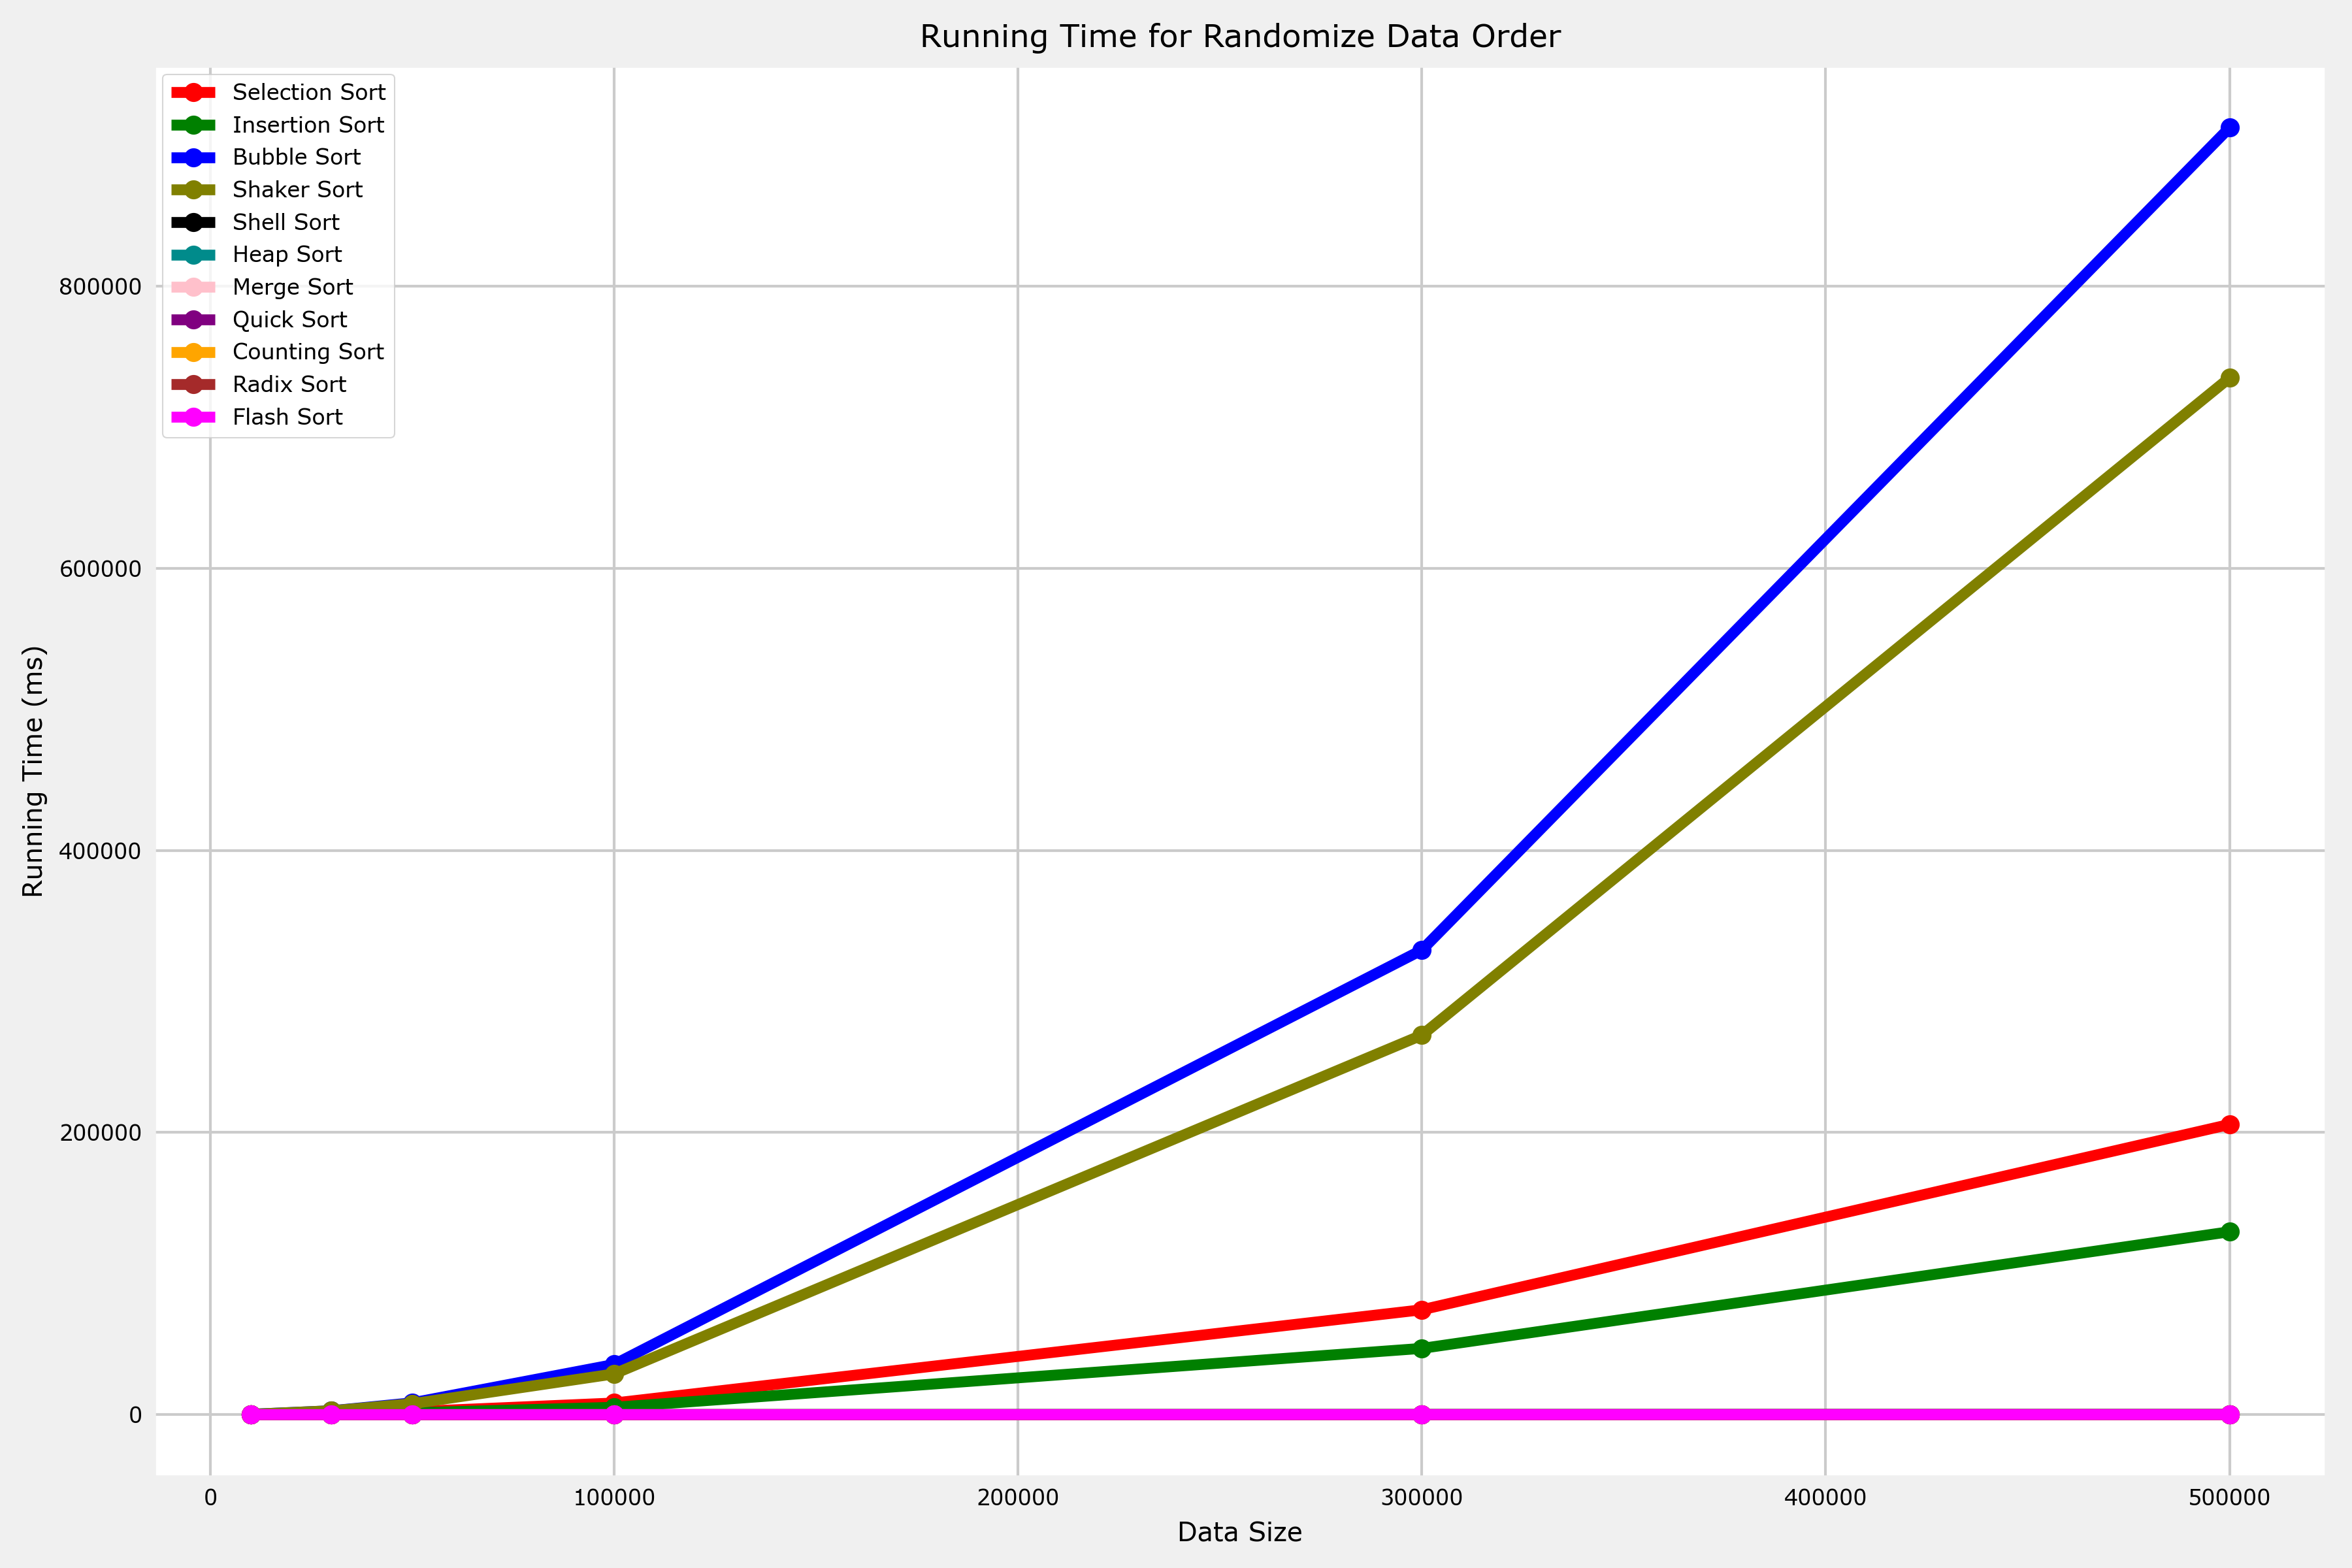
\includegraphics[width=\textwidth]{experimental_result/images/randomize_running_time.png}
    \caption{Thời gian chạy của 11 thuật toán với dữ liệu ngẫu nhiên}
    \label{fig:randomize_running_time}
\end{figure}


\begin{figure}[H]
    \centering
    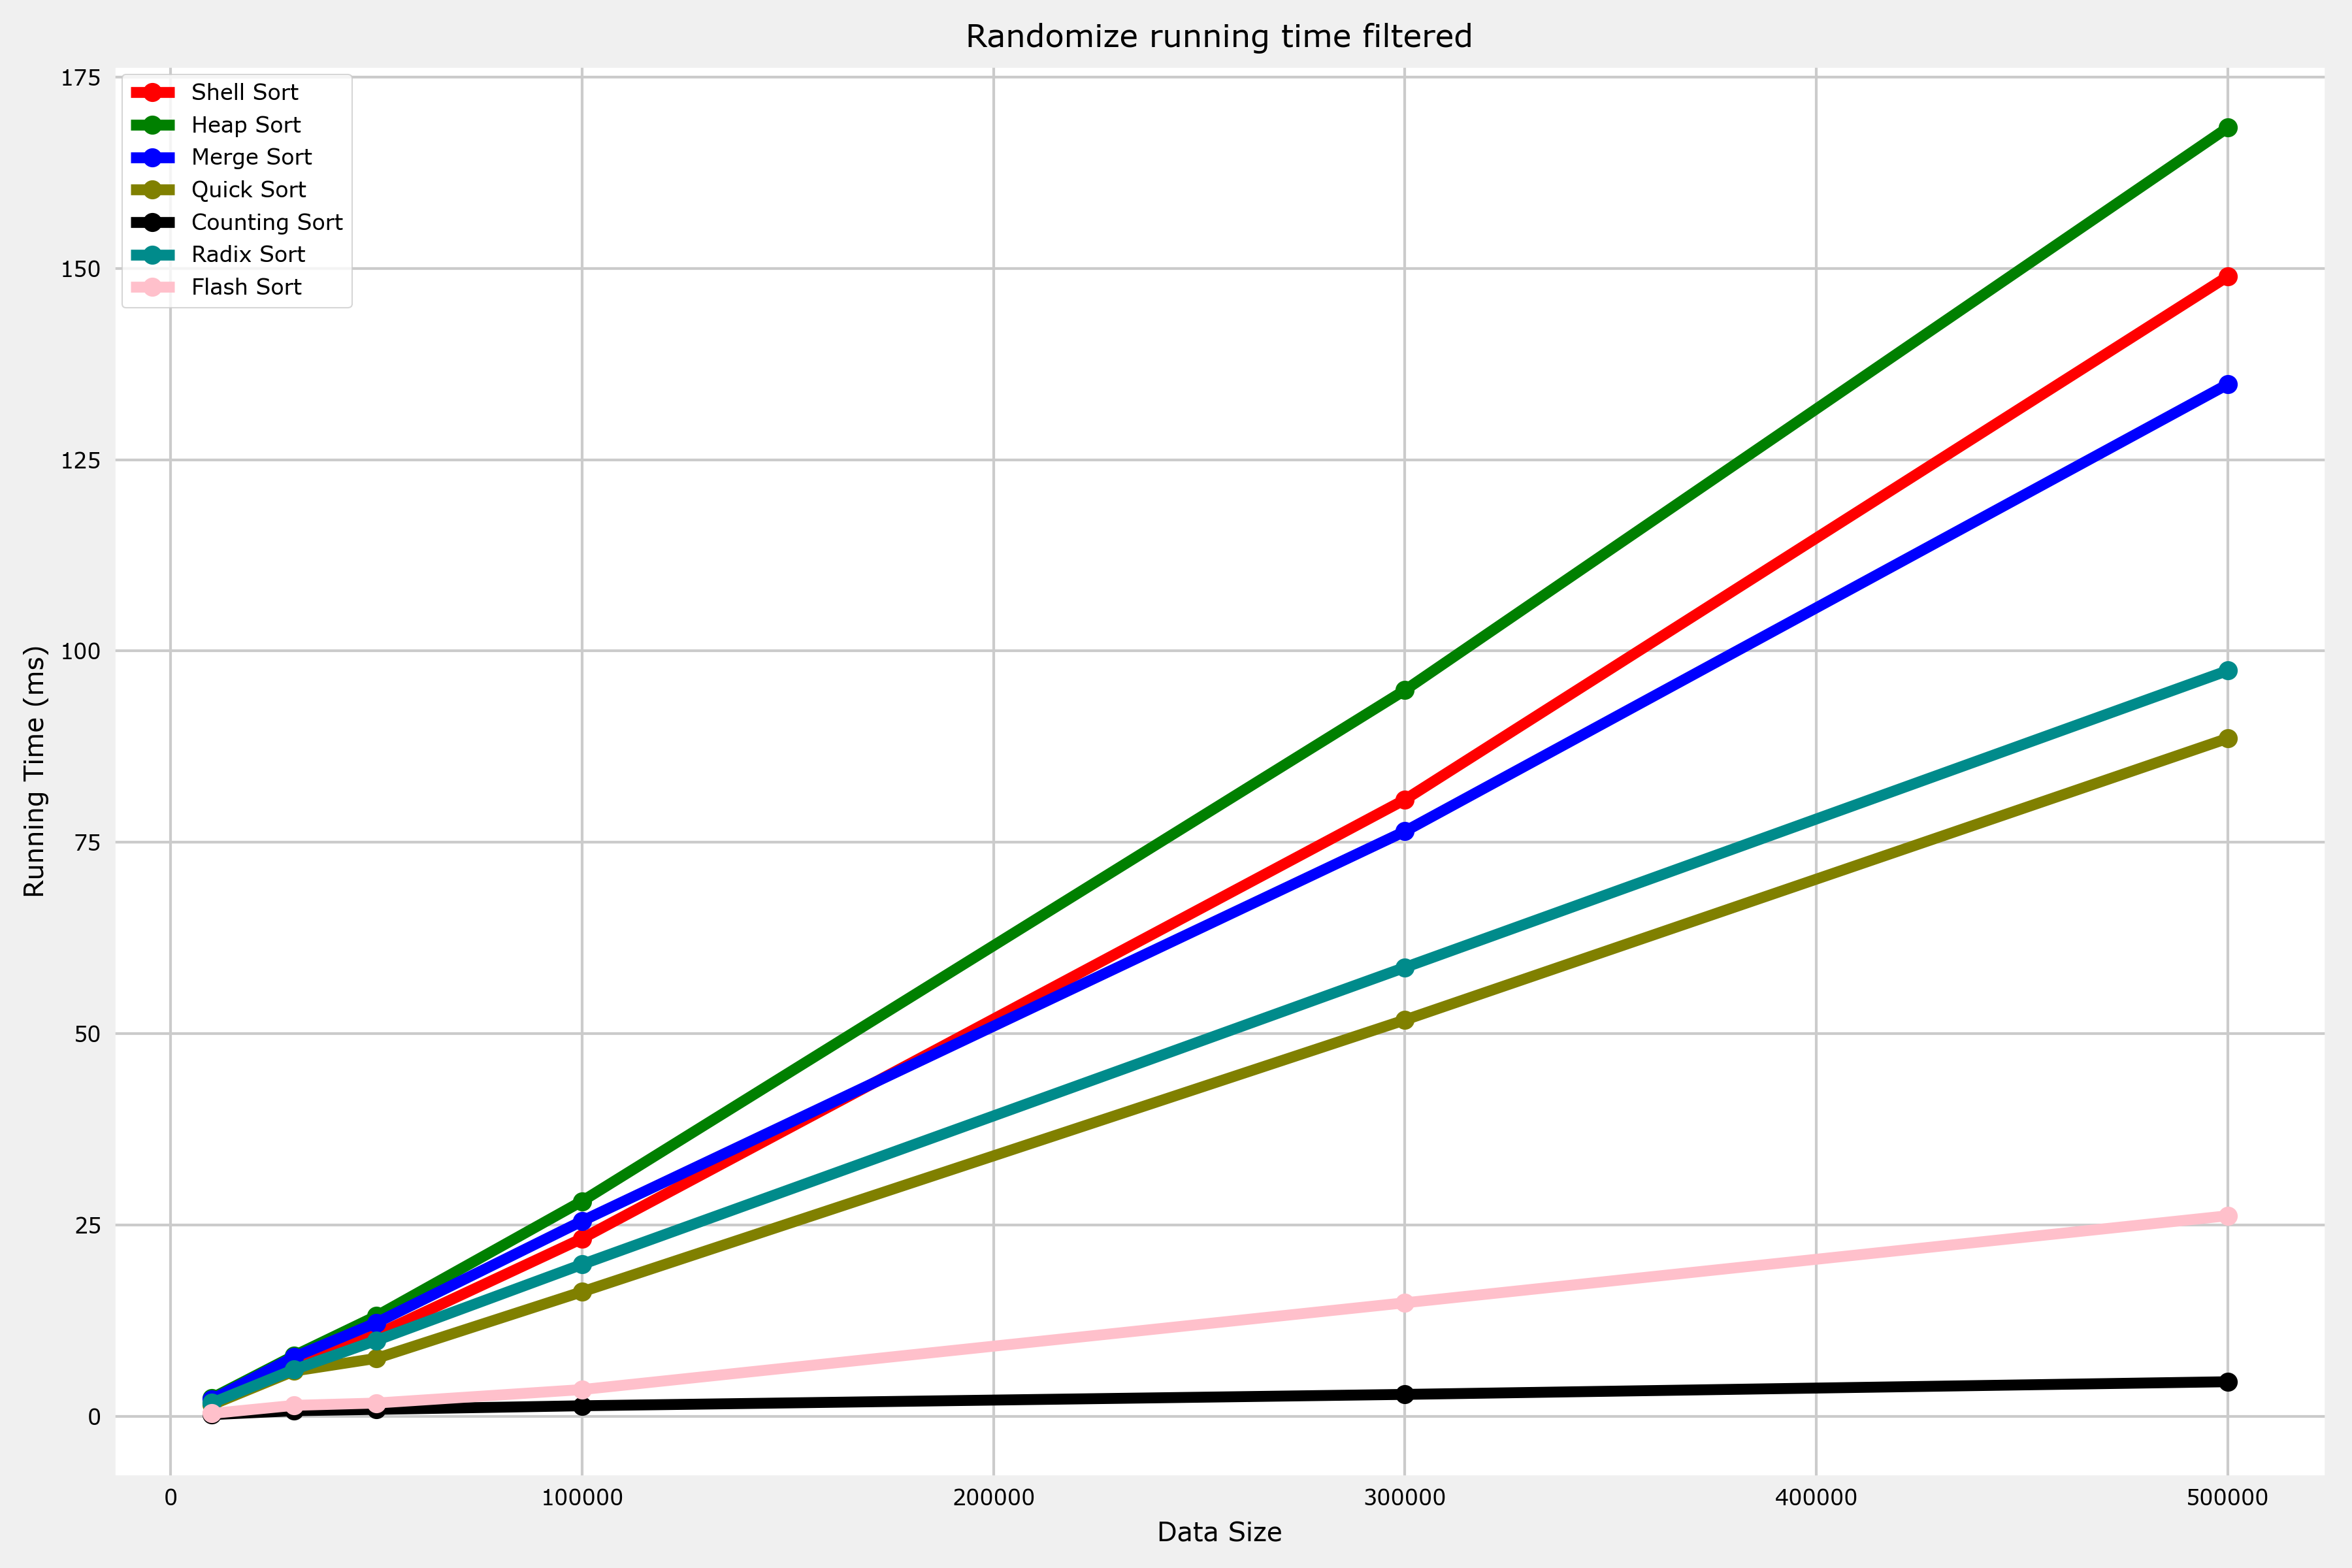
\includegraphics[width=\textwidth]{experimental_result/images/randomize_running_time_filtered.png}
    \caption{Thời gian chạy của 11 thuật toán với dữ liệu ngẫu nhiên sau khi loại bỏ outlier}
    \label{fig:randomize_running_time_filtered}
\end{figure}

Các thuật toán này có xu hướng tuyến tính hơn so với nhóm trước. Thuật toán Counting Sort và Flash Sort là hai thuật toán nhanh nhất, trong khi nhóm các thuật toán cải tiến có thời gian chạy cao hơn nhưng vẫn ổn định. Đặc biệt, Counting Sort có thời gian chạy rất nhỏ các tất cả trường hợp, đều bé hơn $5 ms$ (đường màu đen nằm rất gần trục hoành).




\begin{figure}[H]
    \centering
    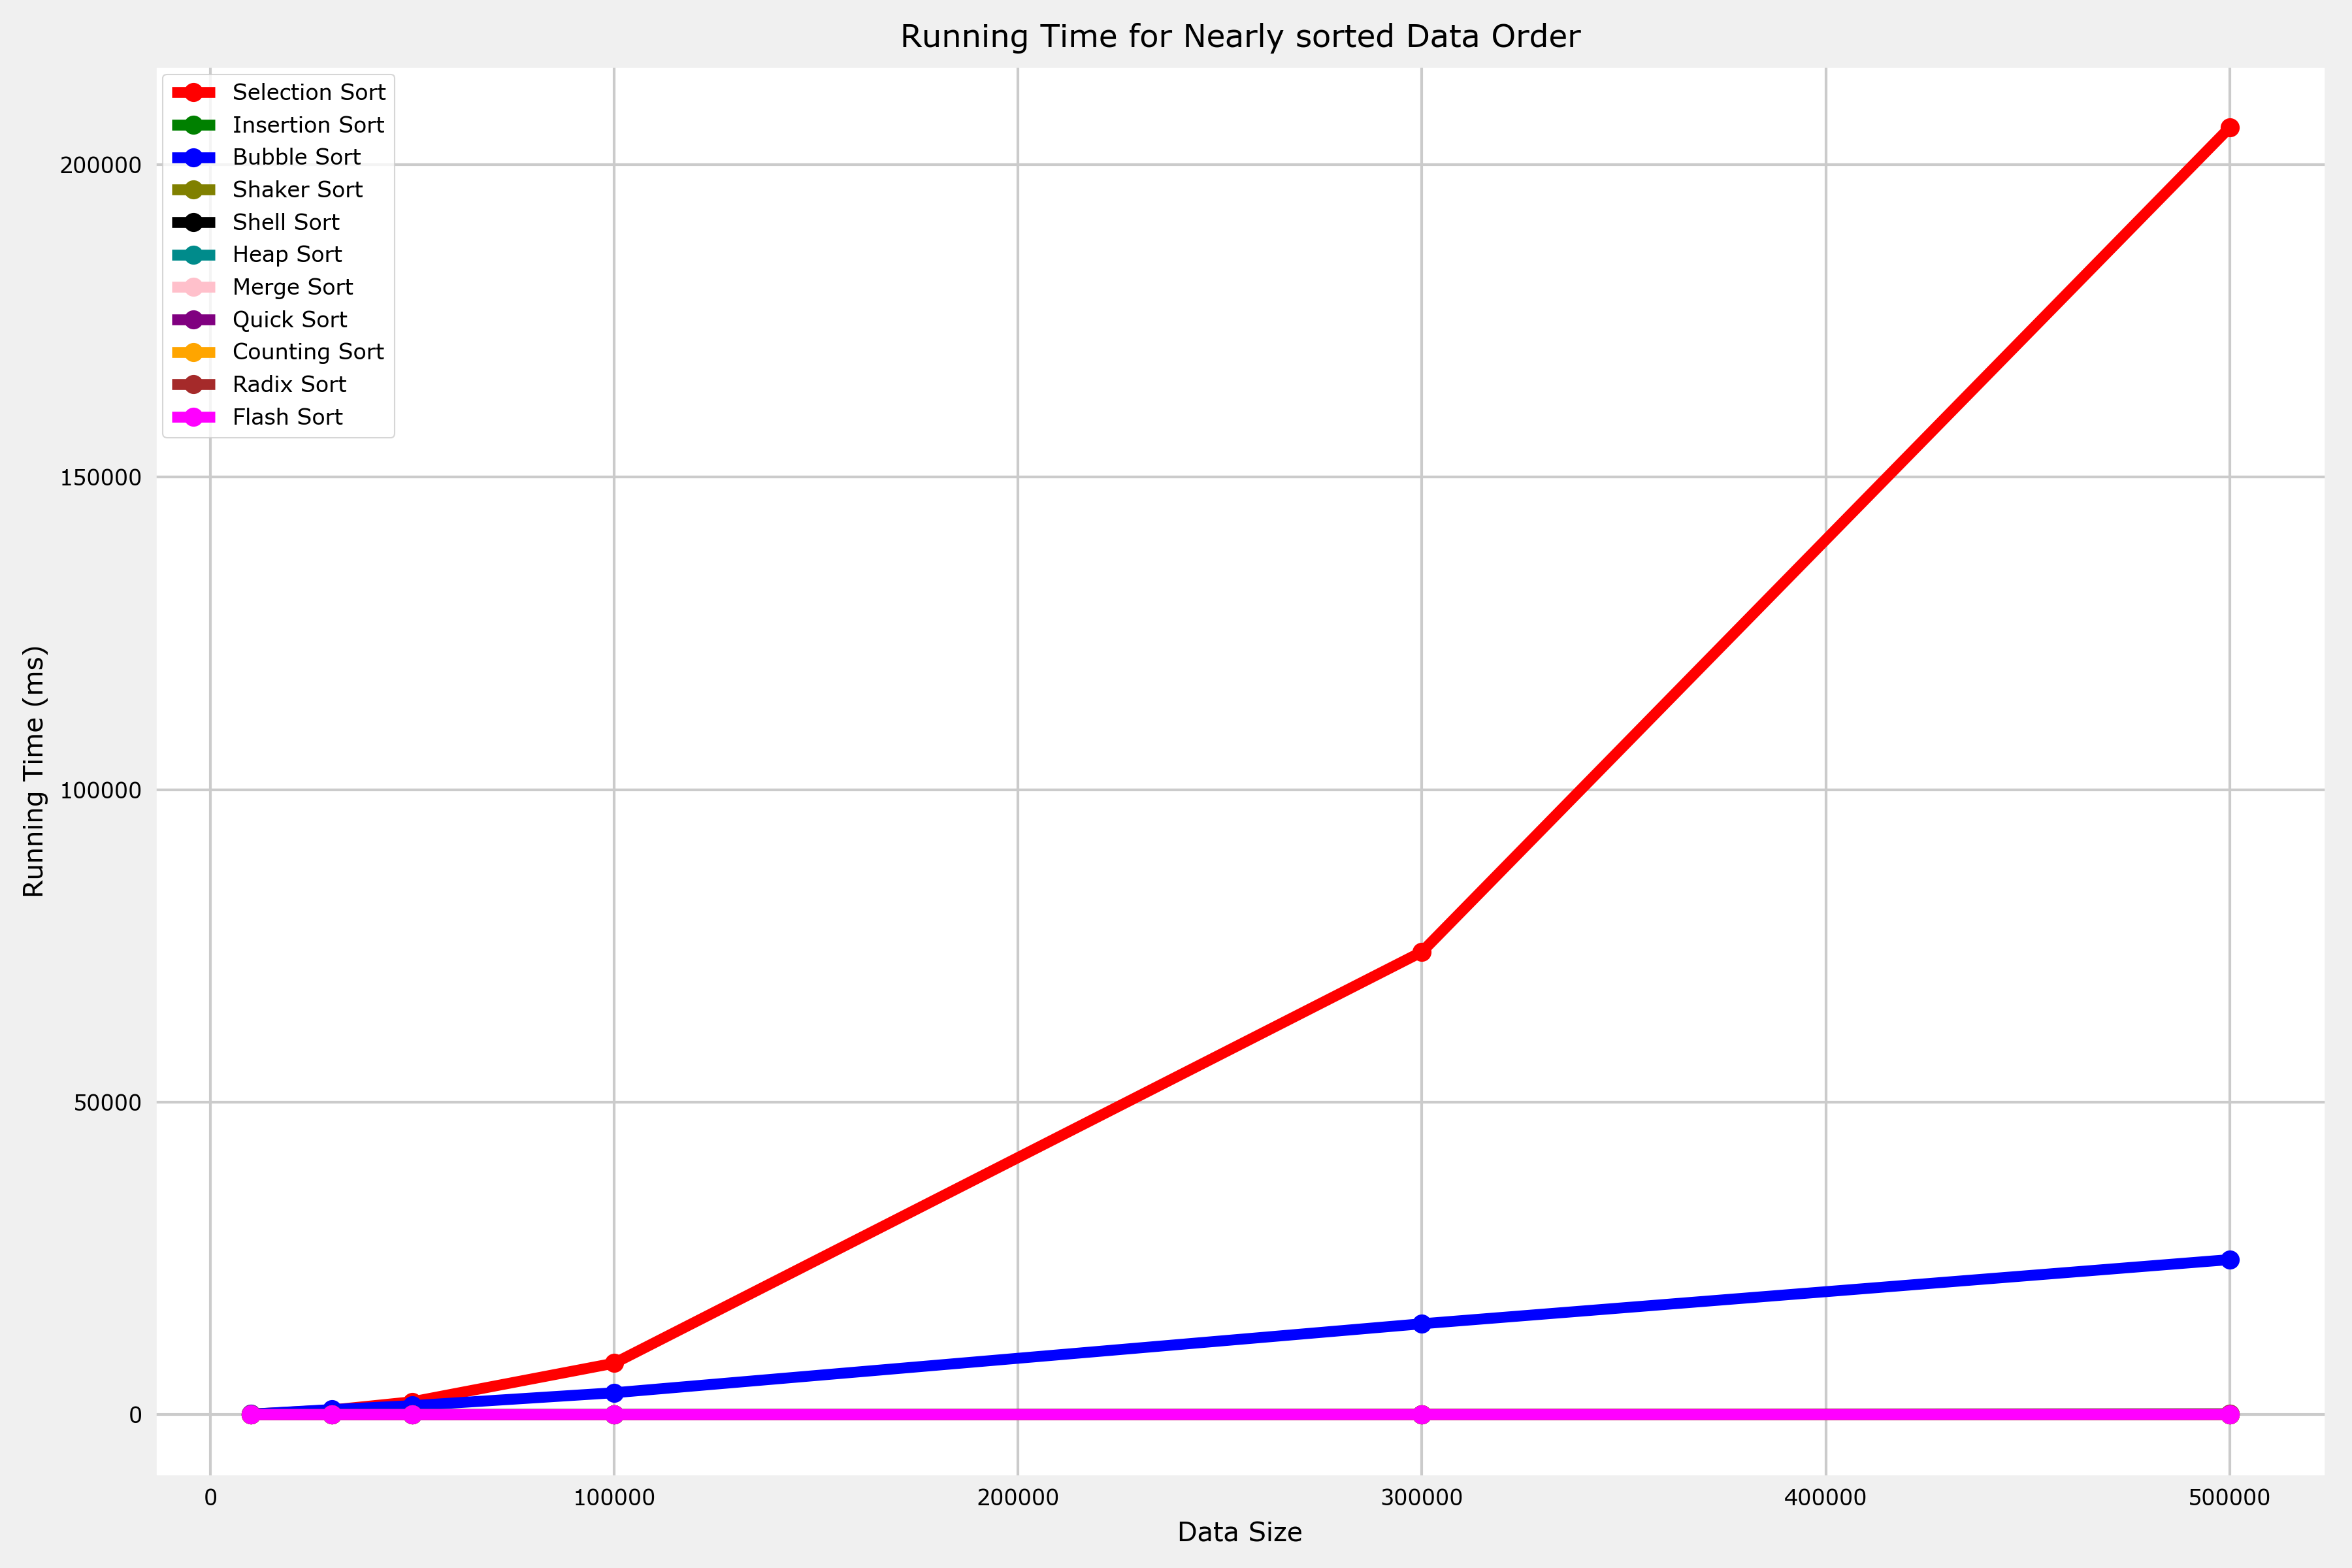
\includegraphics[width=\textwidth]{experimental_result/images/nearly_sorted_running_time.png}
    \caption{Thời gian chạy của 11 thuật toán với dữ liệu gần sắp xếp hoàn chỉnh}
    \label{fig:nearly_sorted_running_time}
\end{figure}
\textbf{3.2.1.2. Dữ liệu gần sắp xếp hoàn chỉnh}


Selection Sort có màn thể hiện rất tệ với dữ liệu gần sắp xếp hoàn chỉnh. Hình \ref{fig:nearly_sorted_running_time} thể hiện rõ độ phức tạp $O(n^2)$ của Selection Sort, tăng rất mạnh khi kích thước dữ liệu lên tới 500.000 phần tử. Thời gian chạy của Bubble Sort tốt hơn Selection Sort nhưng vẫn không tốt bằng các thuật toán khác. Các thuật toán còn lại không thể nhìn thấy do thời gian chạy của chúng nhanh hơn rất nhiều so với Selection Sort. Tiến hành loại bỏ Selection Sort và Bubble Sort, kết quả như hình \ref{fig:nearly_sorted_running_time_filtered}.


\begin{figure}[H]
    \centering
    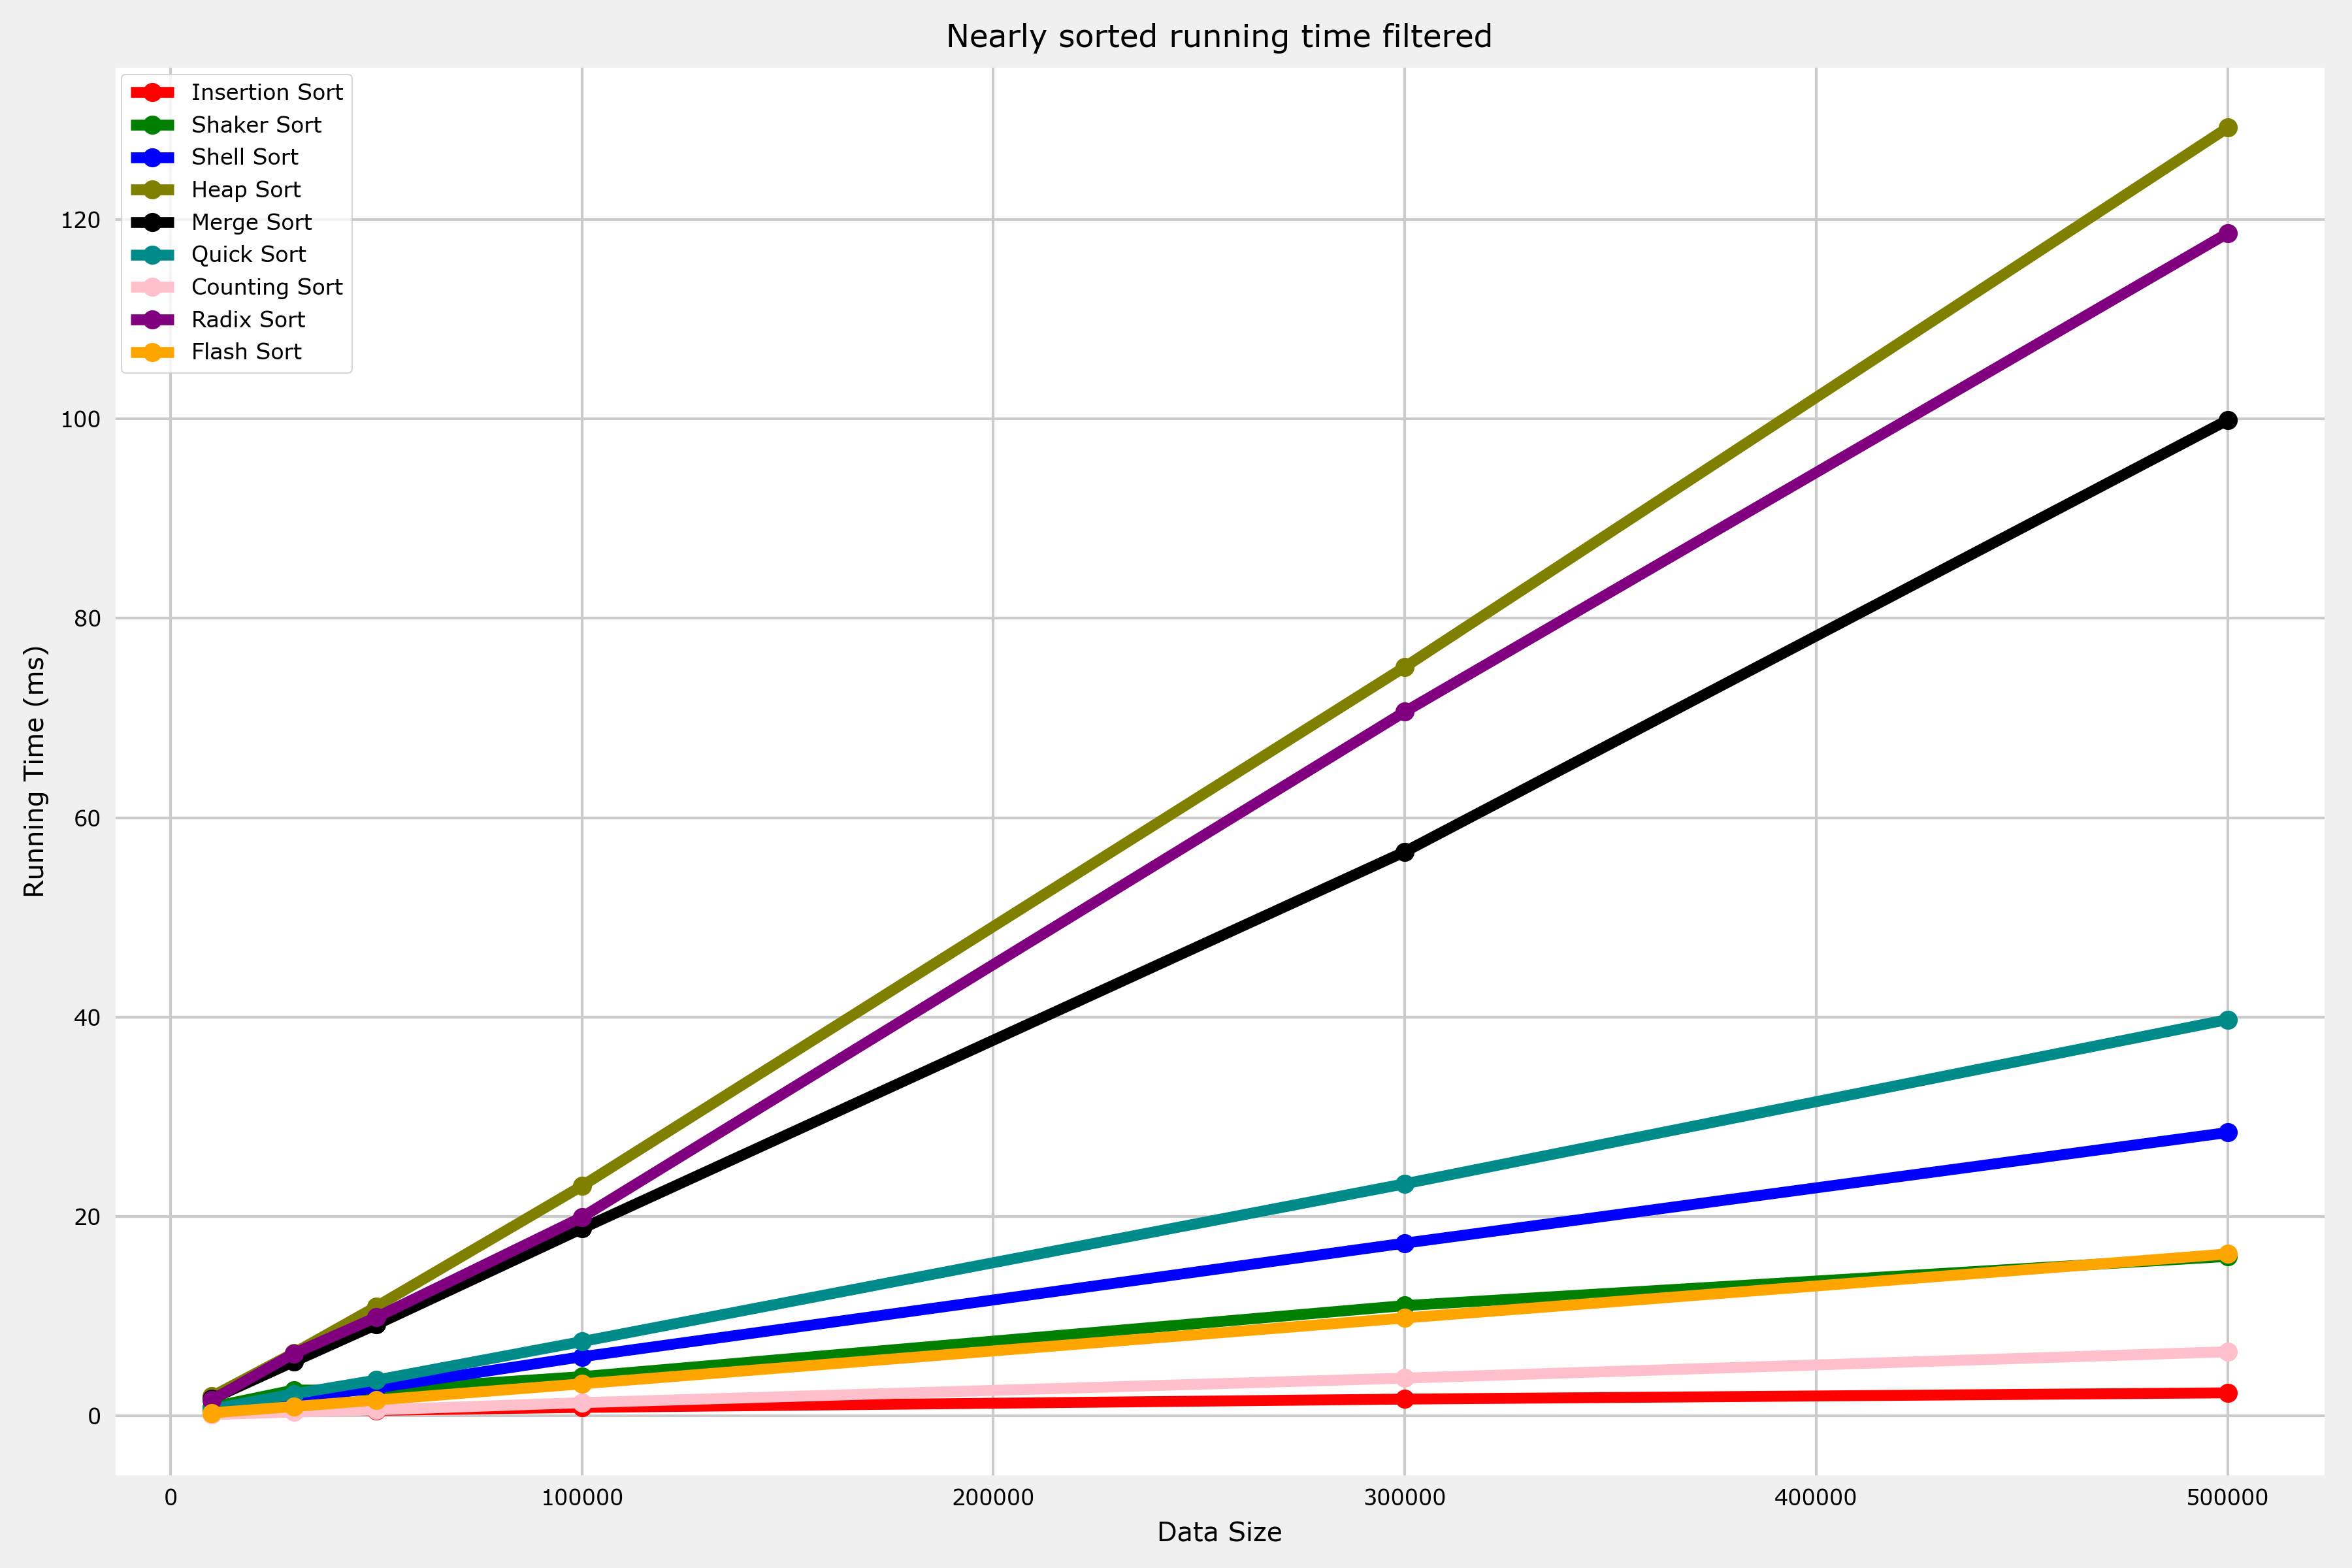
\includegraphics[width=\textwidth]{experimental_result/images/nearly_sorted_running_time_filtered.png}
    \caption{Thời gian chạy của 11 thuật toán với dữ liệu gần sắp xếp hoàn chỉnh sau khi loại bỏ outlier}
    \label{fig:nearly_sorted_running_time_filtered}
\end{figure}

Biểu đồ \ref{fig:nearly_sorted_running_time_filtered} lúc này có xu hướng chia thành hai nhóm nhóm 1 (Heap Sort, Radix Sort, Merge Sort) và nhóm 2, nhanh hơn (Quick Sort, Shell Sort, Shaker Sort, Flash Sort, Counting Sort, Insertion) .Insertion Sort có thời gian thực thi nhanh nhất với bộ dữ liệu này. Điều này khá phù hợp với trường hợp tốt nhất của Insertion Sort là dữ liệu đã sắp xếp. Shaker Sort tốt hơn nhiều so với Bubble Sort và xấp xỉ Flash Sort. Các thuật toán cải tiến và không sắp xếp khá ổn định giống như bộ dữ liệu trước.



\begin{figure}[H]
    \centering
    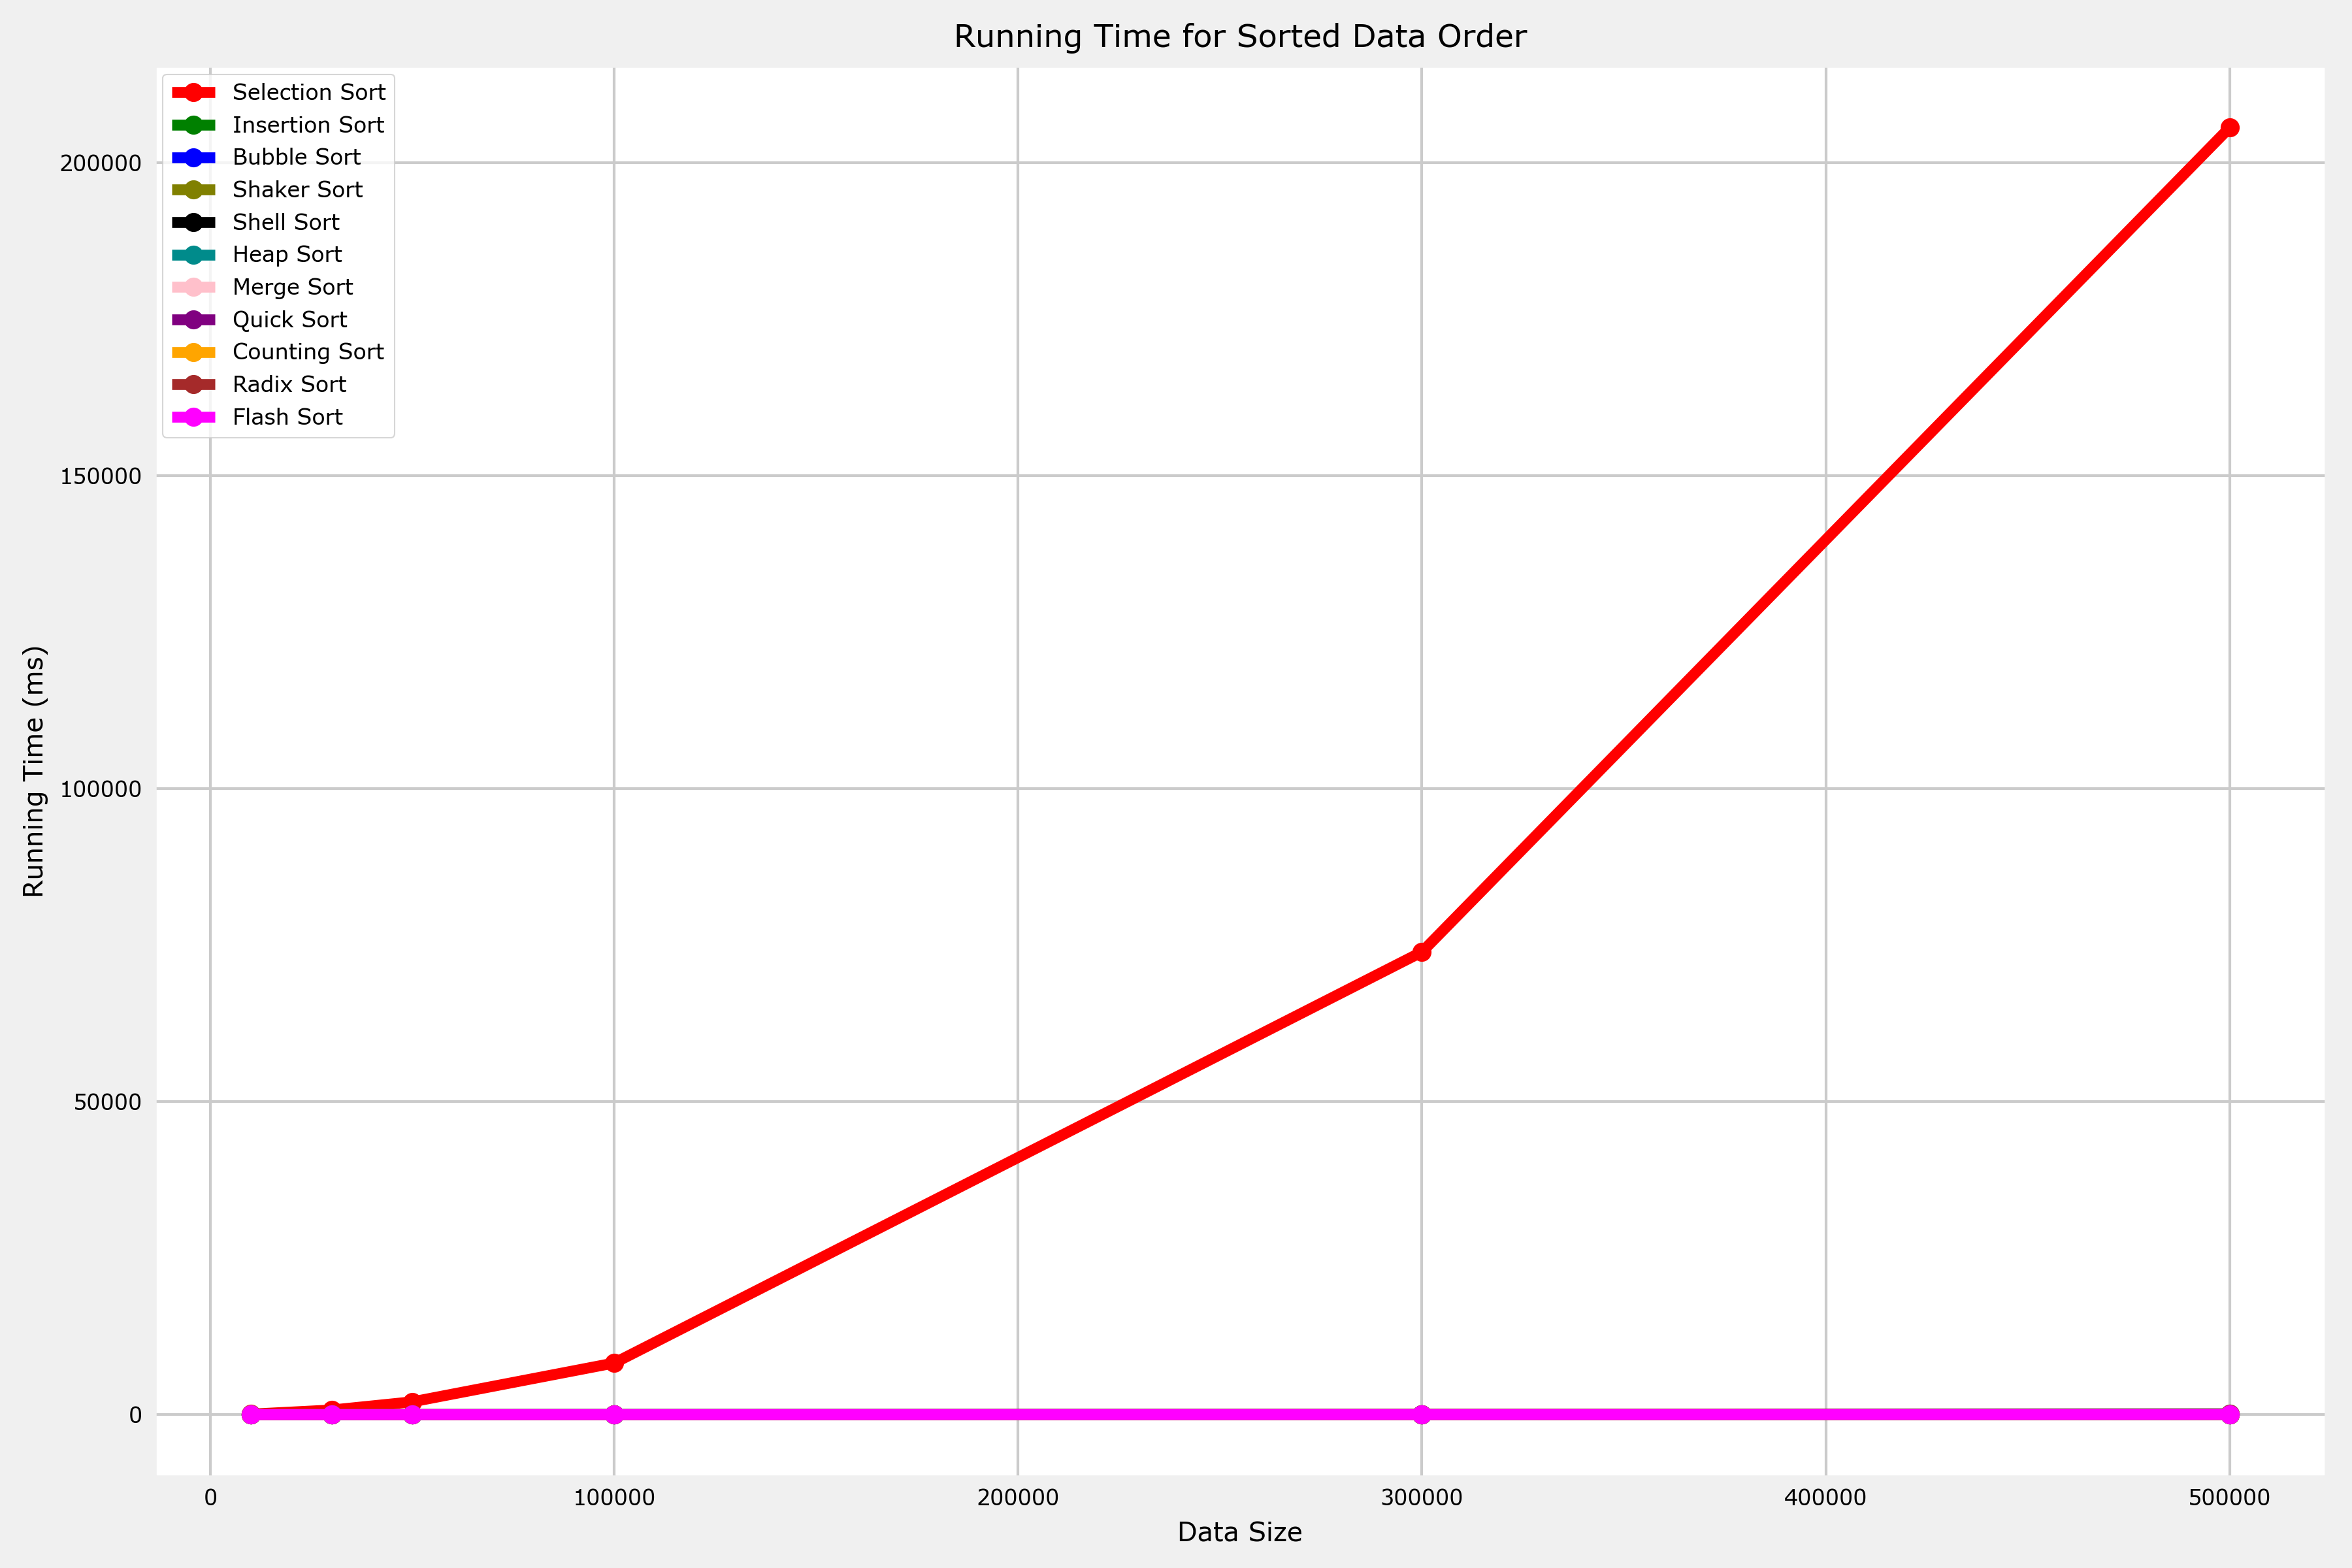
\includegraphics[width=\textwidth]{experimental_result/images/sorted_running_time.png}
    \caption{Thời gian chạy của 11 thuật toán với dữ liệu được sắp xếp}
    \label{fig:sorted_running_time}
\end{figure}

\textbf{3.2.1.3. Dữ liệu được sắp xếp}

Selection vẫn có thời gian thực thi lớn so với các thuật toán còn lại như trên hình \ref{fig:sorted_running_time}. Tiếp tục tách Selection Sort ra khỏi biểu đồ.

\begin{figure}[H]
    \centering
    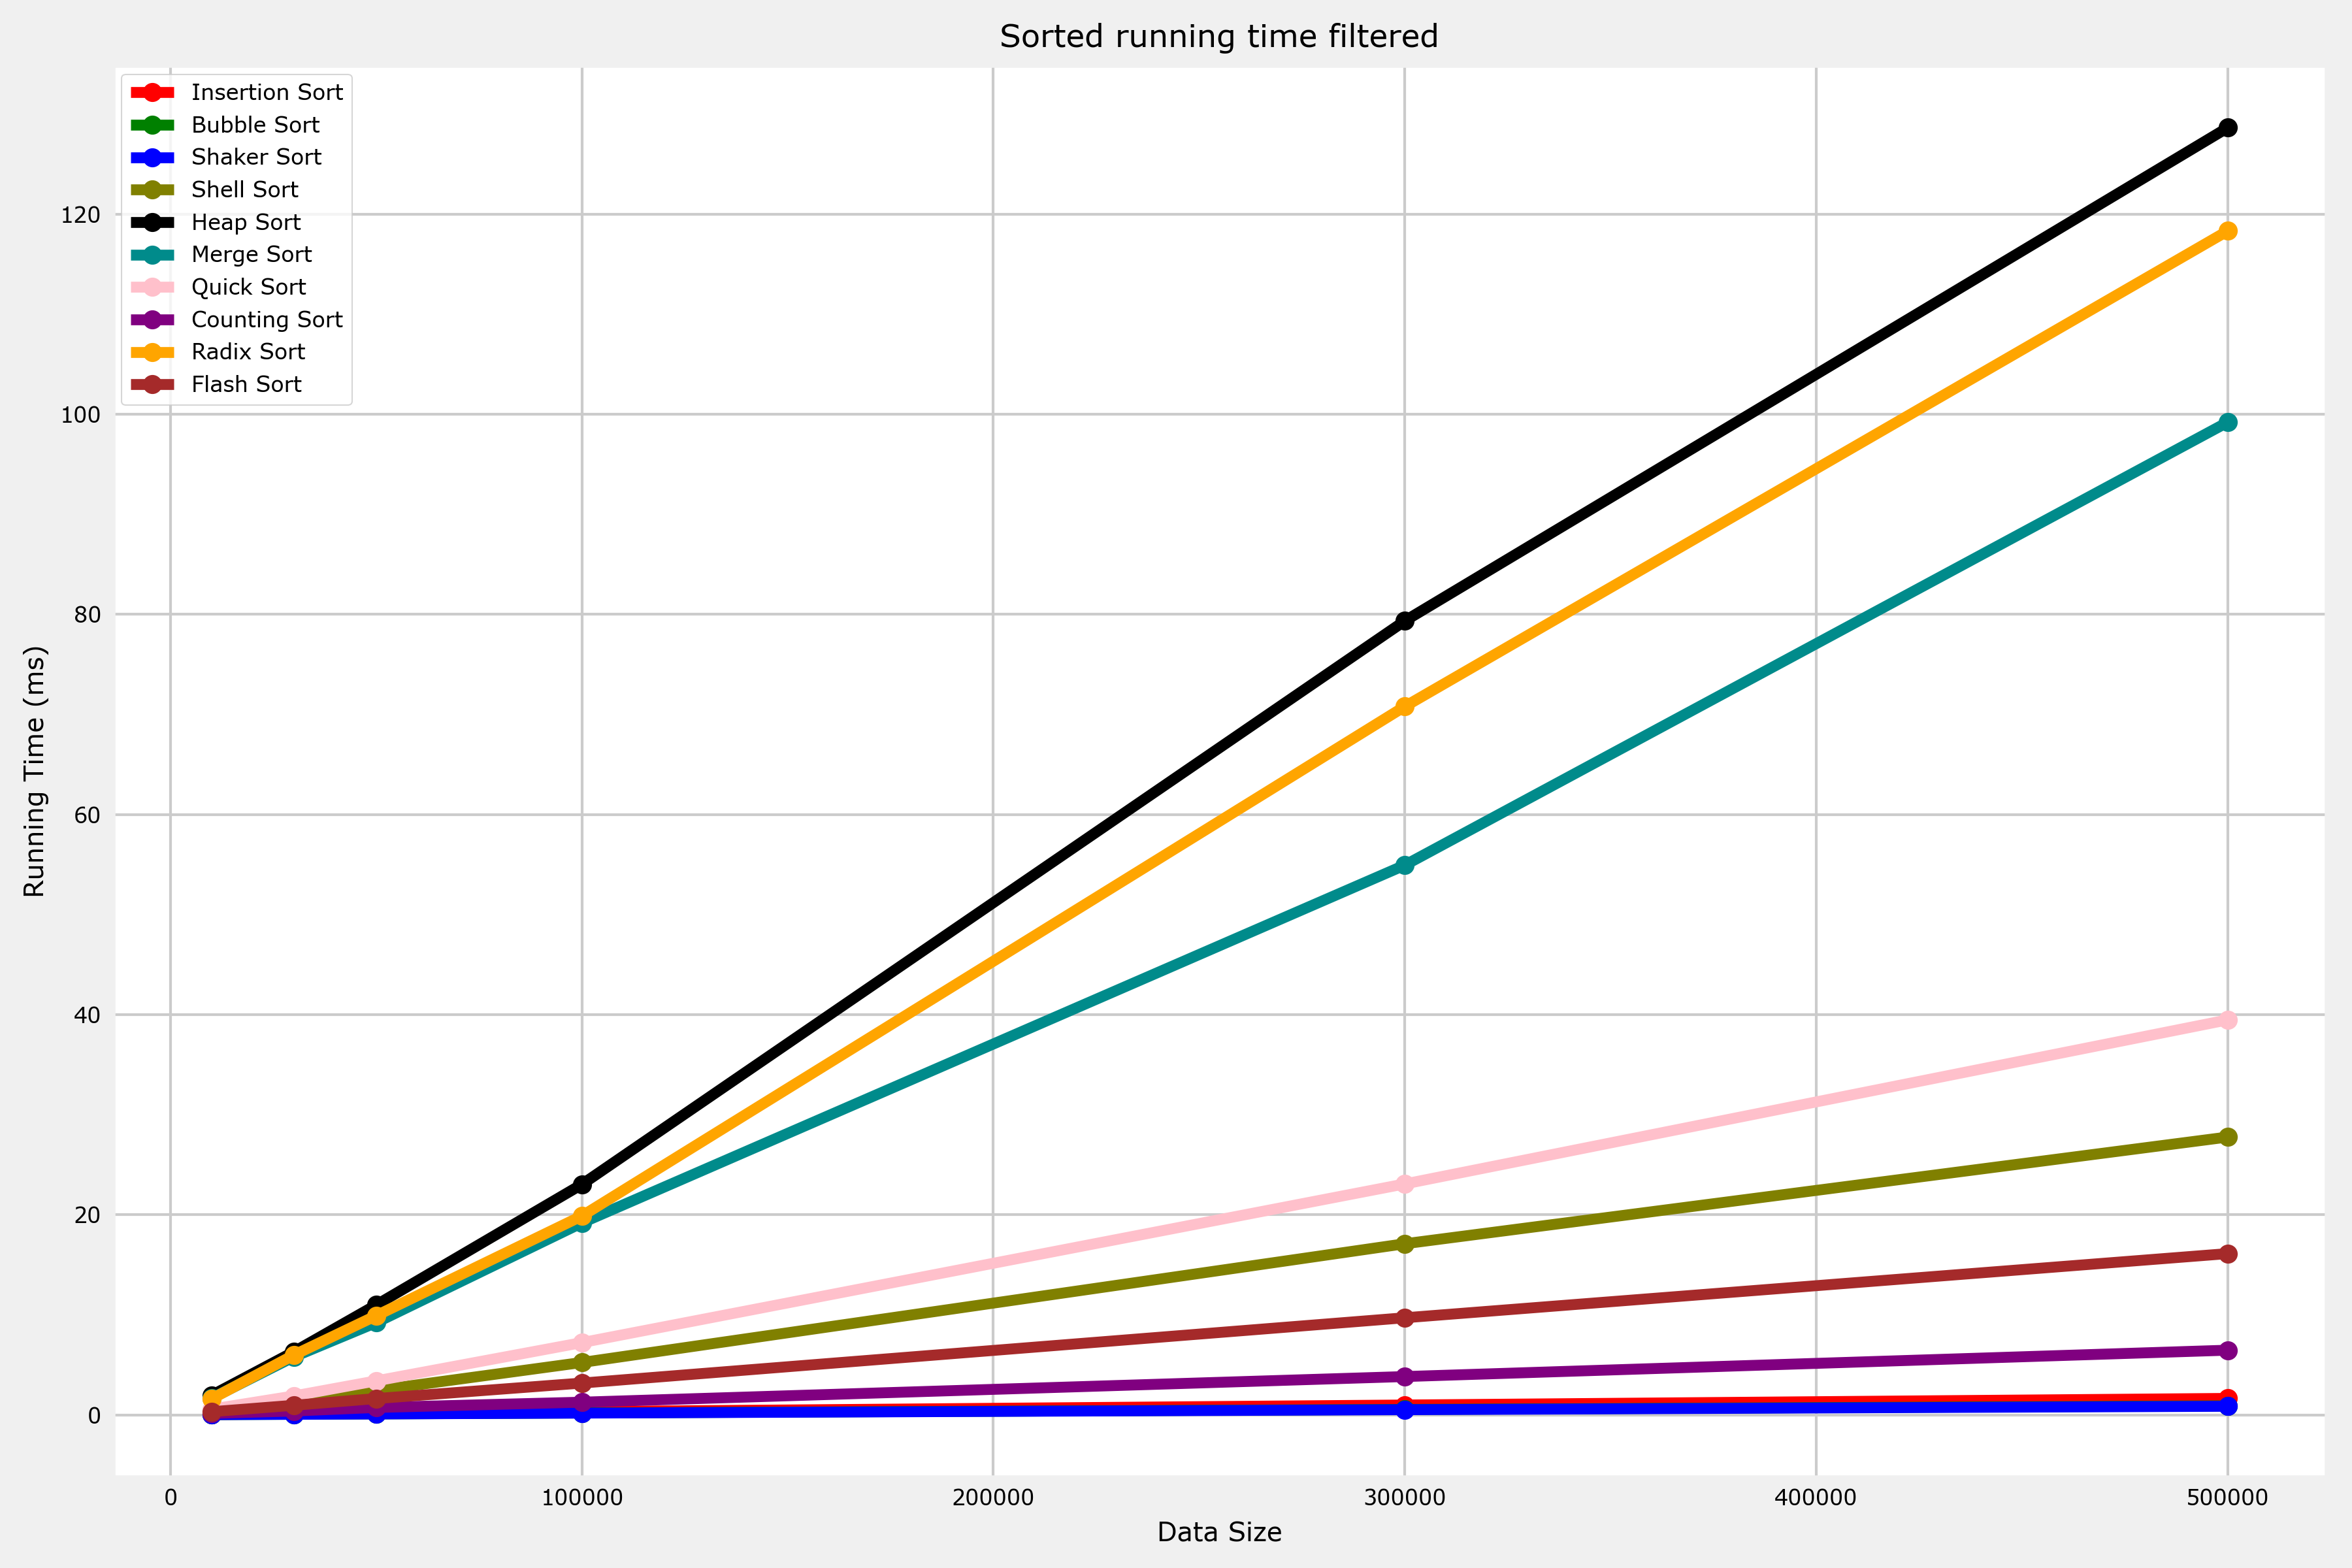
\includegraphics[width=\textwidth]{experimental_result/images/sorted_running_time_filtered.png}
    \caption{Thời gian chạy của 11 thuật toán với dữ liệu được sắp xếp sau khi loại bỏ outlier}
    \label{fig:sorted_running_time_filtered}
\end{figure}

Có hai nhóm thuật toán chính trên biểu đồ \ref{fig:sorted_running_time_filtered}: nhóm 1 (Heap Sort, Radix Sort, Merge Sort) và nhóm 2 (các thuật toán còn lại). Nhóm 1 vẫn giống như trên bộ dữ liệu gần sắp xếp hoàn chỉnh, tương đối ổn định. Nhóm 2 có tốc độ tăng thời gian chạy theo của kích thước của dữ liệu chậm hơn so với nhóm 1. Shaker Sort và Insertion Sort là hai thuật toán nhanh nhất. Bộ dữ liệu này chính là trường hợp tốt nhất cho độ phức tạp thời gian của hai thuật toán này và bằng $\Theta(n)$.


\begin{figure}[H]
    \centering
    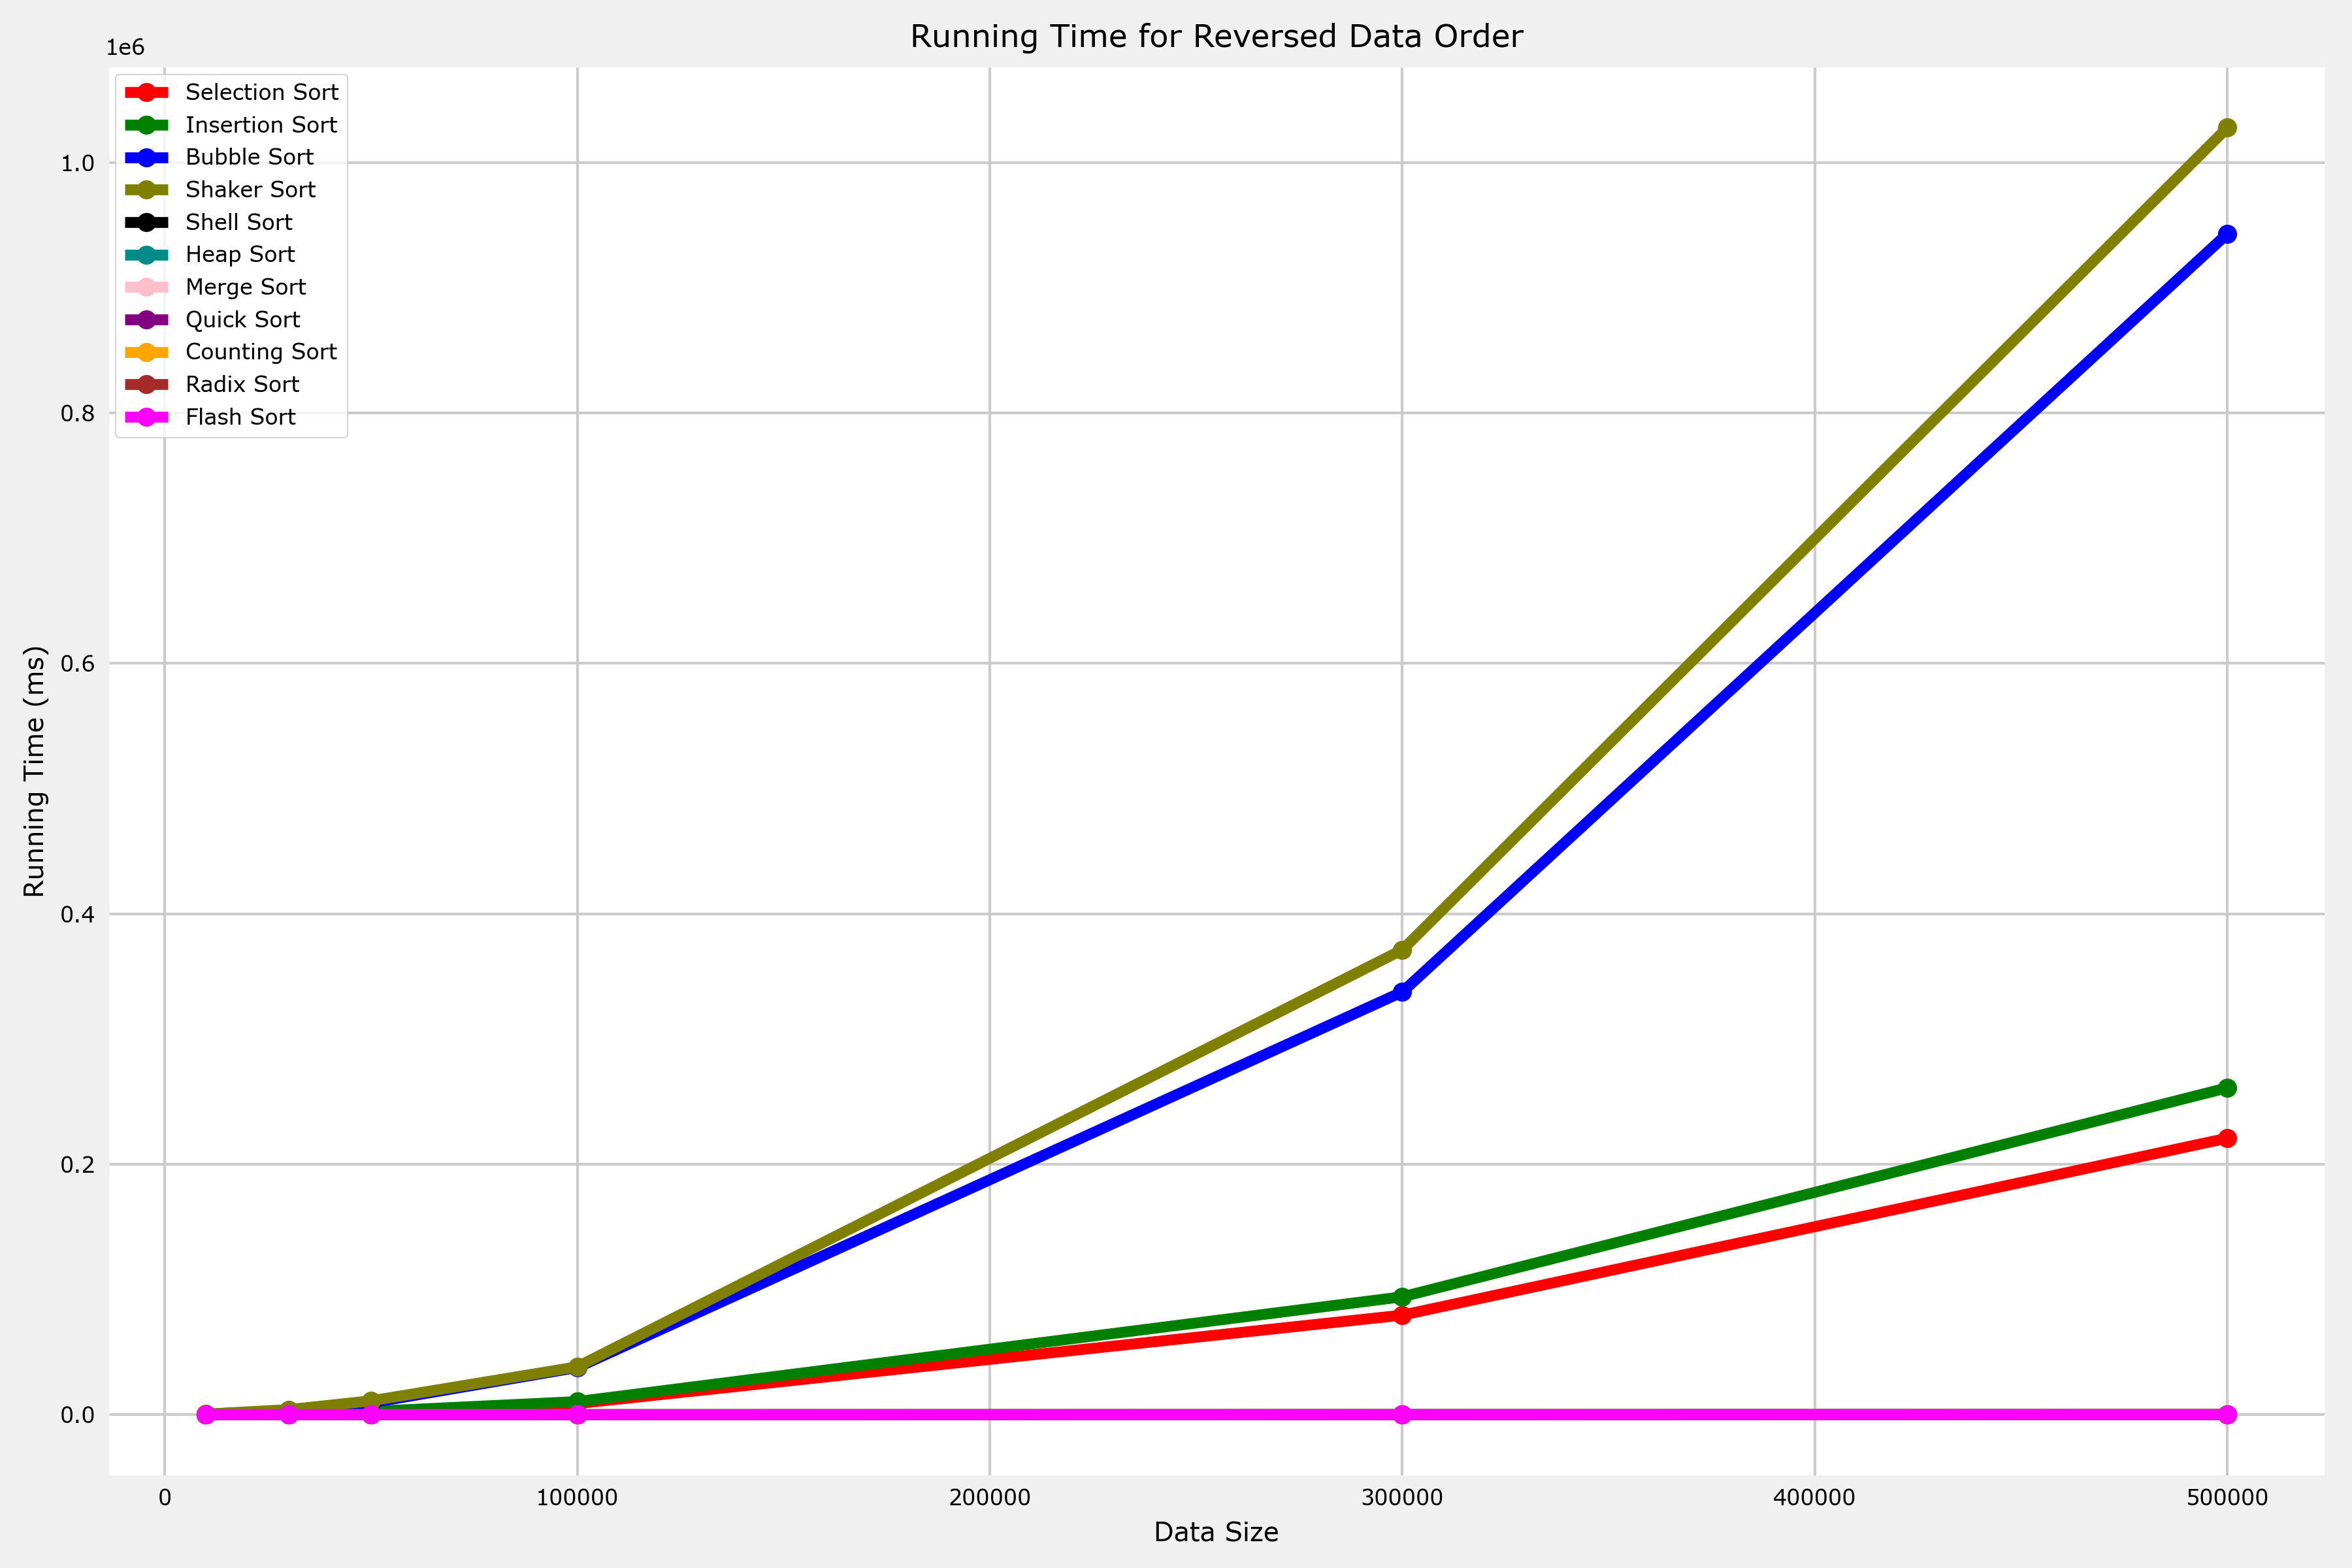
\includegraphics[width=\textwidth]{experimental_result/images/reversed_running_time.png}
    \caption{Thời gian chạy của 11 thuật toán với dữ liệu đảo ngược}
    \label{fig:reversed_running_time}
\end{figure}

\textbf{3.2.1.4. Dữ liệu đảo ngược}


Đối với bộ dữ liệu đảo ngược, Shaker Sort có thời gian chạy tương đối bằng Bubble Sort. Thời gian thực thi của Selection Sort và Insertion Sort khá giống nhau. Shaker Sort và Bubble Sort thể hiện khuynh hướng tăng mạnh hơn so với Selection Sort và Insertion Sort khi gặp kích thước dữ liệu lớn. Hình \ref{fig:reversed_running_time_filtered} có được sau khi bỏ qua 4 thuật toán nhóm cơ bản.

\begin{figure}[H]
    \centering
    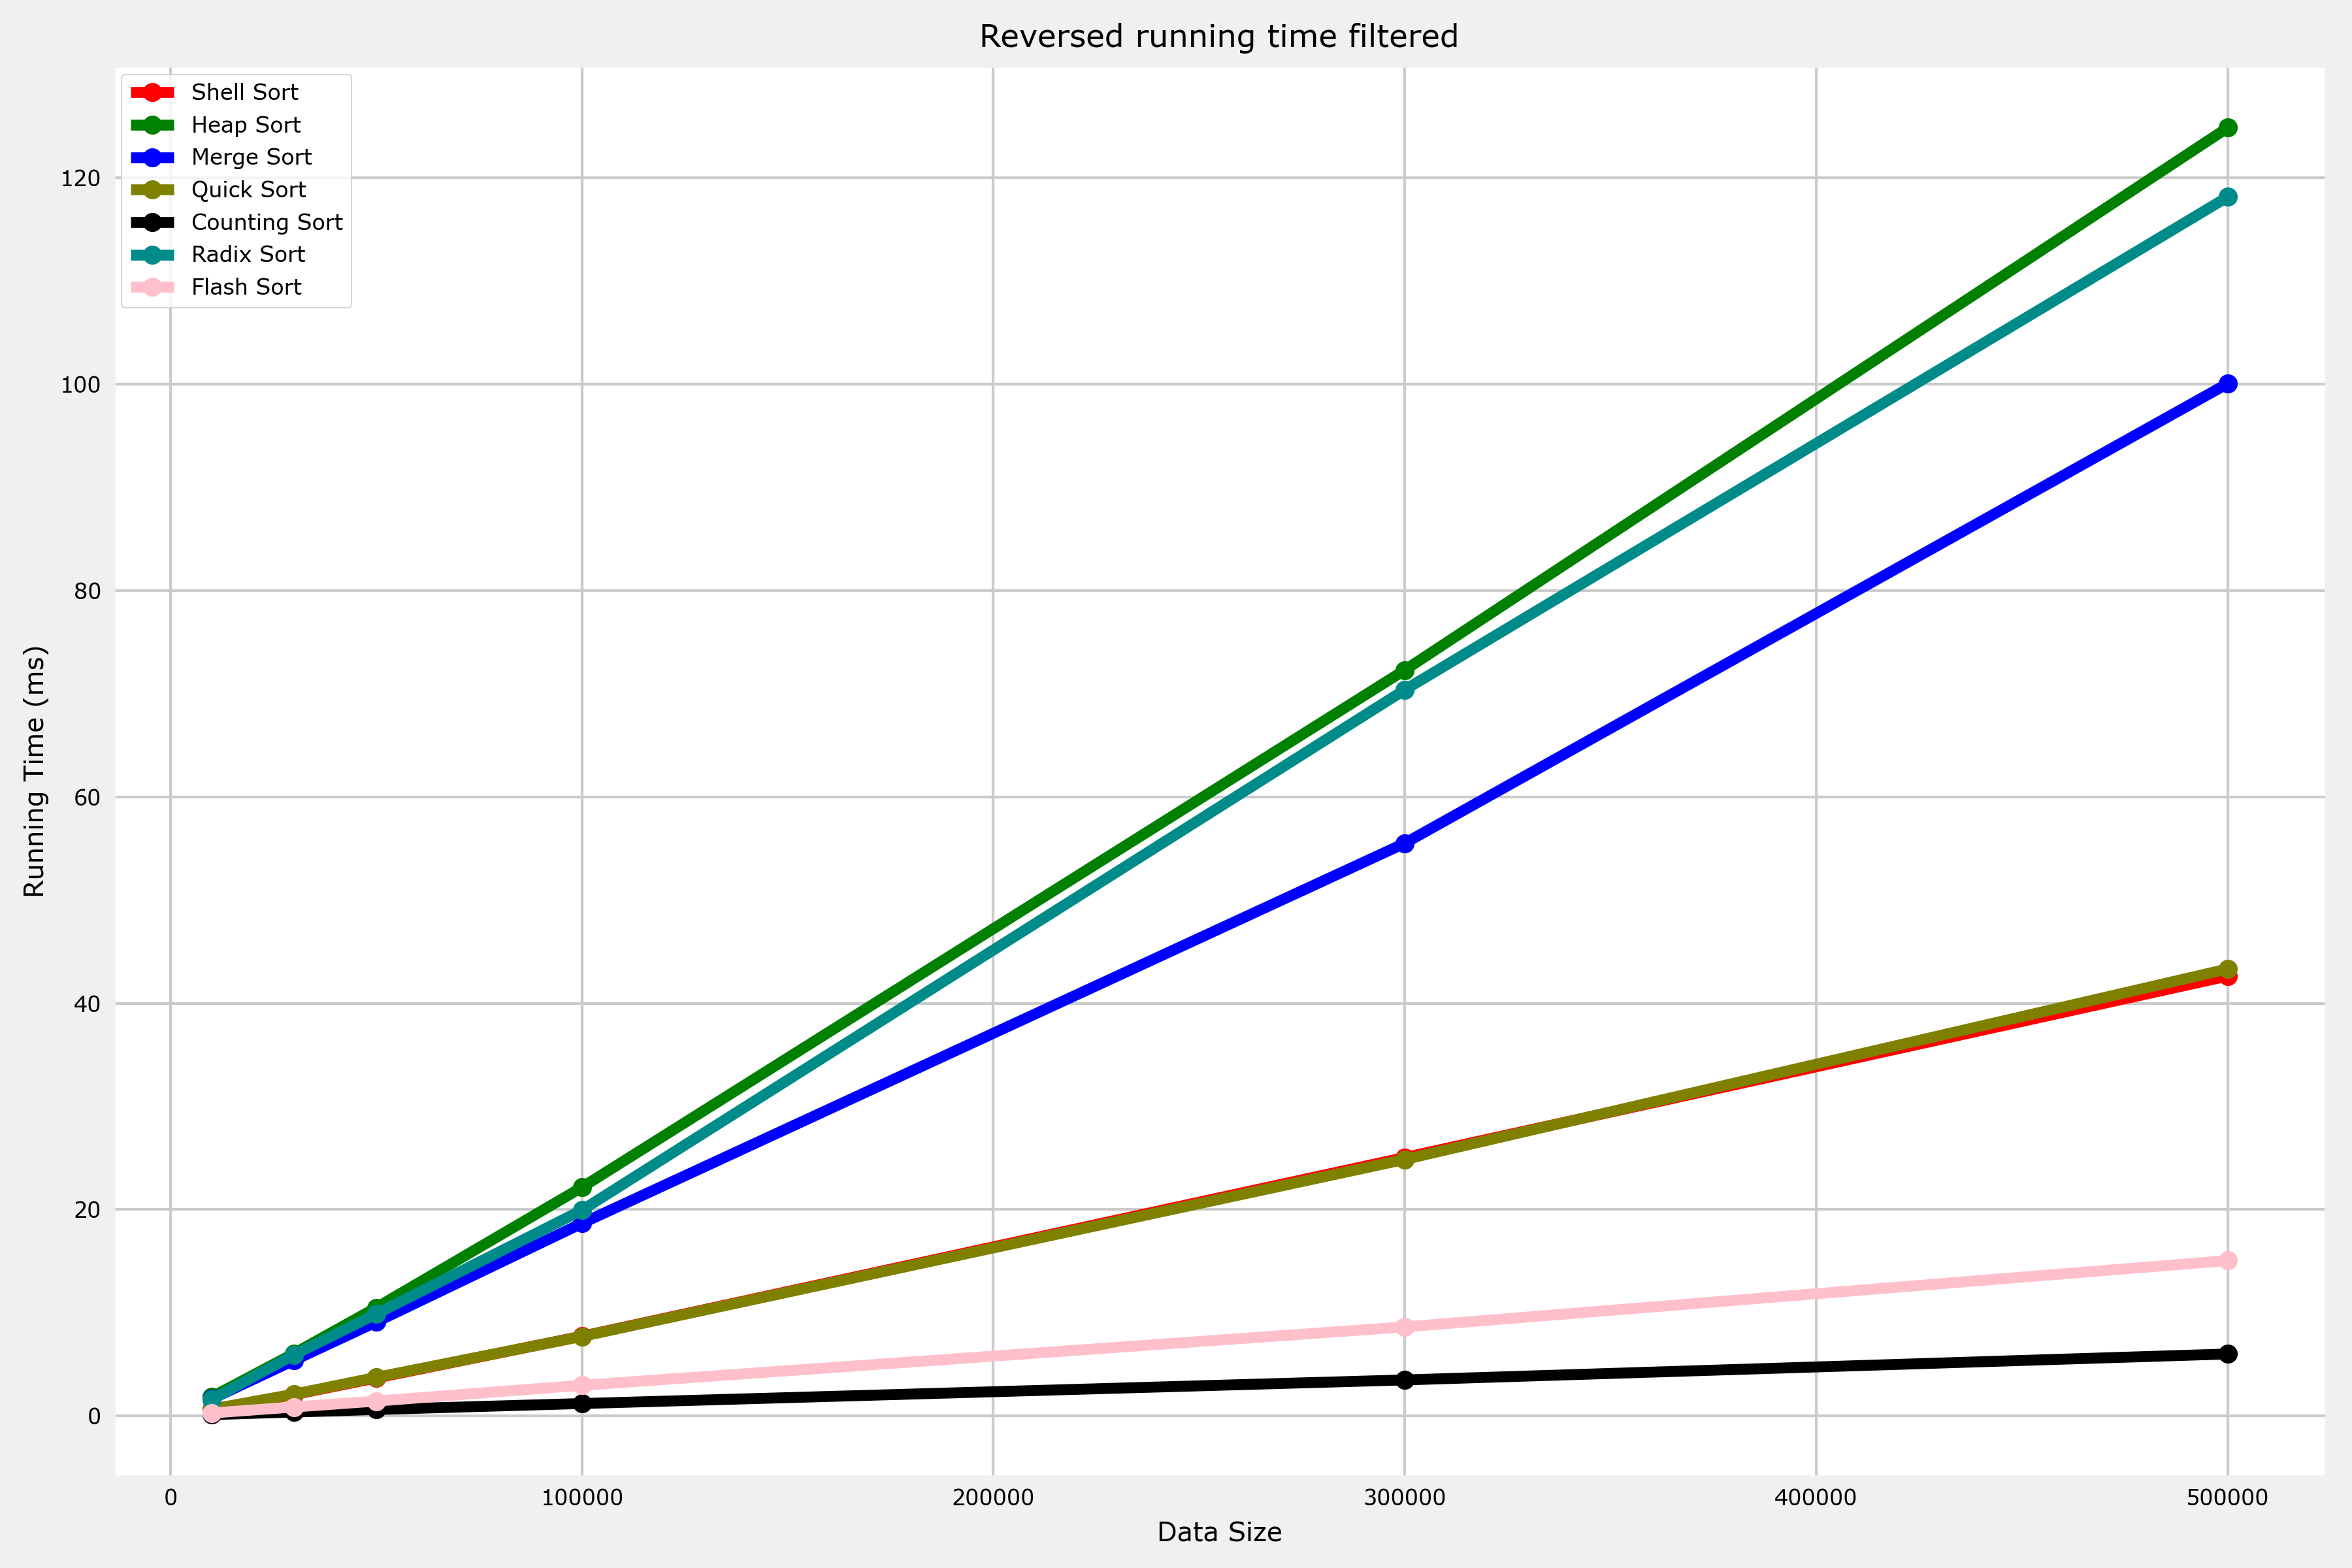
\includegraphics[width=\textwidth]{experimental_result/images/reversed_running_time_filtered.png}
    \caption{Thời gian chạy của 11 thuật toán với dữ liệu đảo ngược sau khi loại bỏ outlier}
    \label{fig:reversed_running_time_filtered}
\end{figure}


Ba thuật toán Heap Sort, Radix Sort, Merge Sort đã thể hiện được tính ổn đỉnh trong cả tất cả trường hợp. Hai thuật toán nhanh nhất vẫn là Counting Sort và Flash Sort. Đường biểu diễn của Quick Sort và Shell Sort khá trùng nhau.








\subsubsection{Biểu đồ số phép so sánh}

Đầu tiên, tiến hành vẽ tất cả biểu đồ trên các thứ tự khác nhau của 11 thuật toán, được hình \ref{fig:all_the_number_of_comparisons_for_each_algorithm_of_each_data_order}.

\begin{figure}[H]
    \centering
    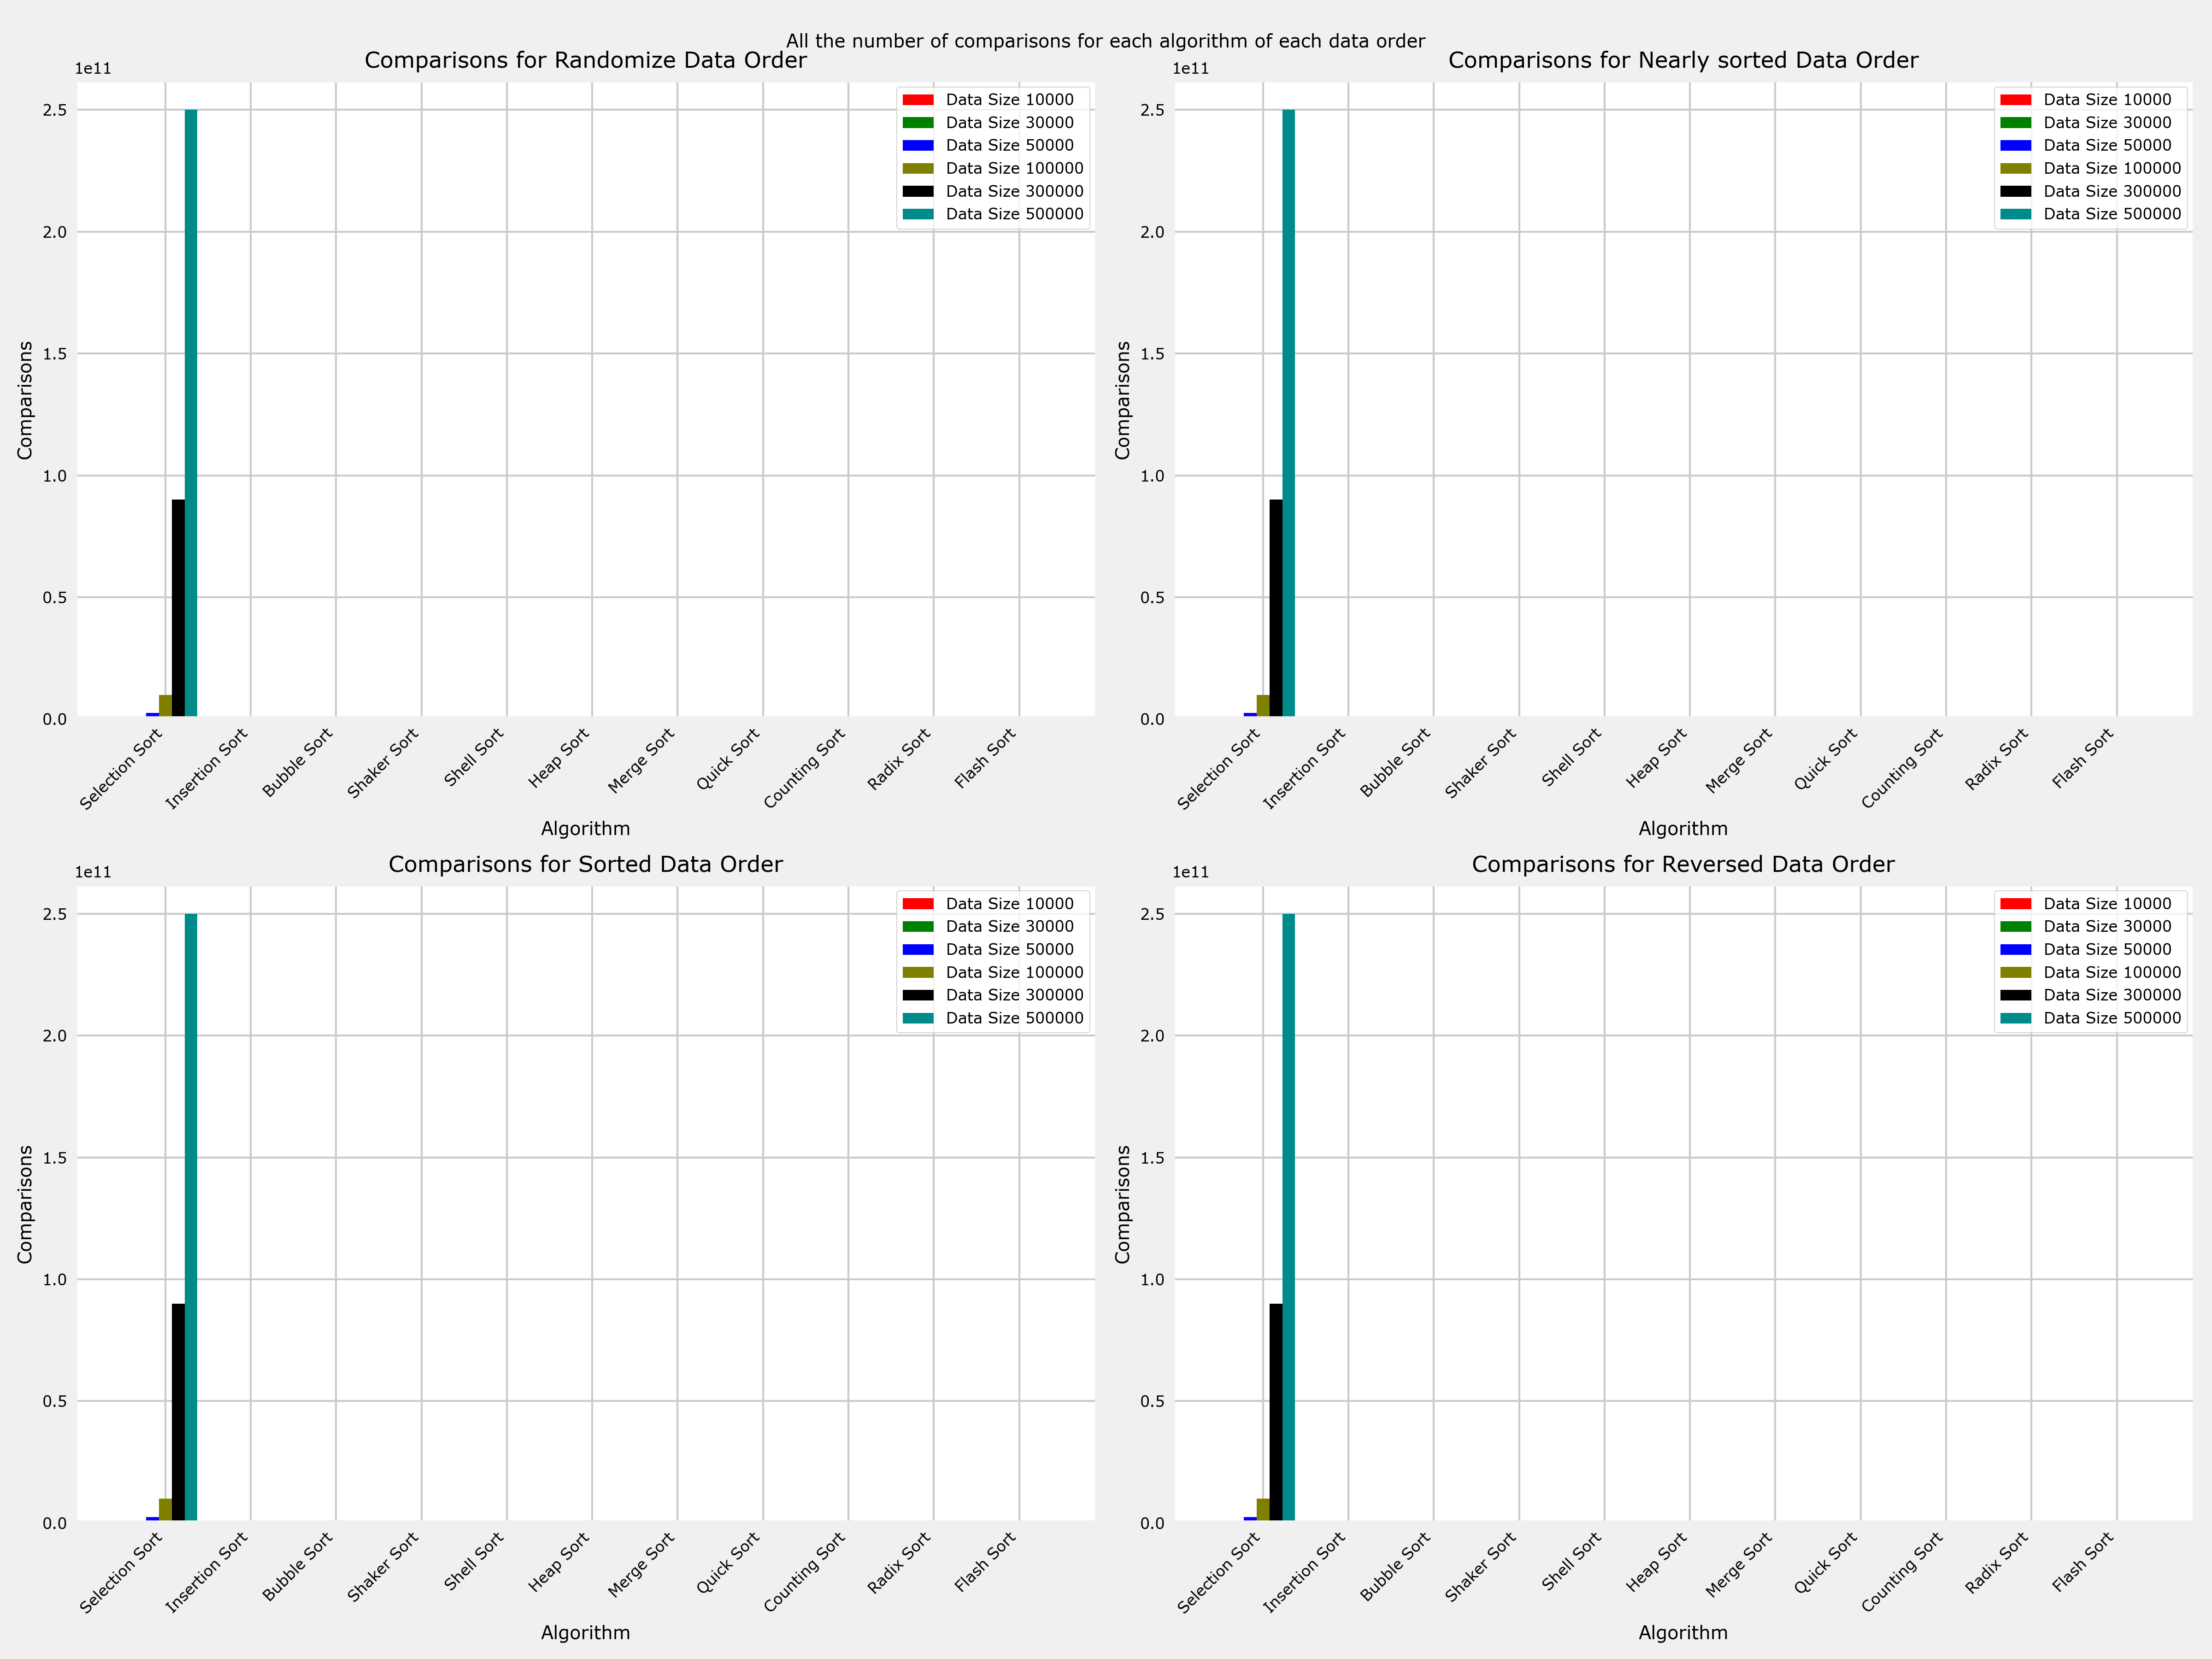
\includegraphics[width=\textwidth]{experimental_result/images/all_the_number_of_comparisons_for_each_algorithm_of_each_data_order.png}
    \caption{Số phép so sánh của 11 thuật toán với tất cả trường hợp của dữ liệu}
    \label{fig:all_the_number_of_comparisons_for_each_algorithm_of_each_data_order}
\end{figure}

Dễ thấy, Selection Sort số lượng phép so sánh vượt trội hơn 10 thuật toán còn lại, và đạt đến 2500049999 phép so sánh. Do đó, các thuật toán còn lại không thể nhìn thấy được trên biểu đồ. Selection Sort tăng rất mạnh khi gặp kích thước dữ liệu tăng dần, thể hiện độ phức tạp thời gian trung bình $\Theta(n^2)$. Vì thuật toán này luôn duyệt tất cả trường hợp có thể xảy ra, không dừng sớm khi đã sắp xếp xong nên số lượng phép so sánh là như nhau đối với tất cả trường hợp của mảng trong thực nghiệm (Phần 3.1 \ref{subsec:experimental_result}).  

Từ đây bỏ qua Selection Sort để thuận tiện cho việc trực quan hóa dữ liệu.


\begin{figure}[H]
    \centering
    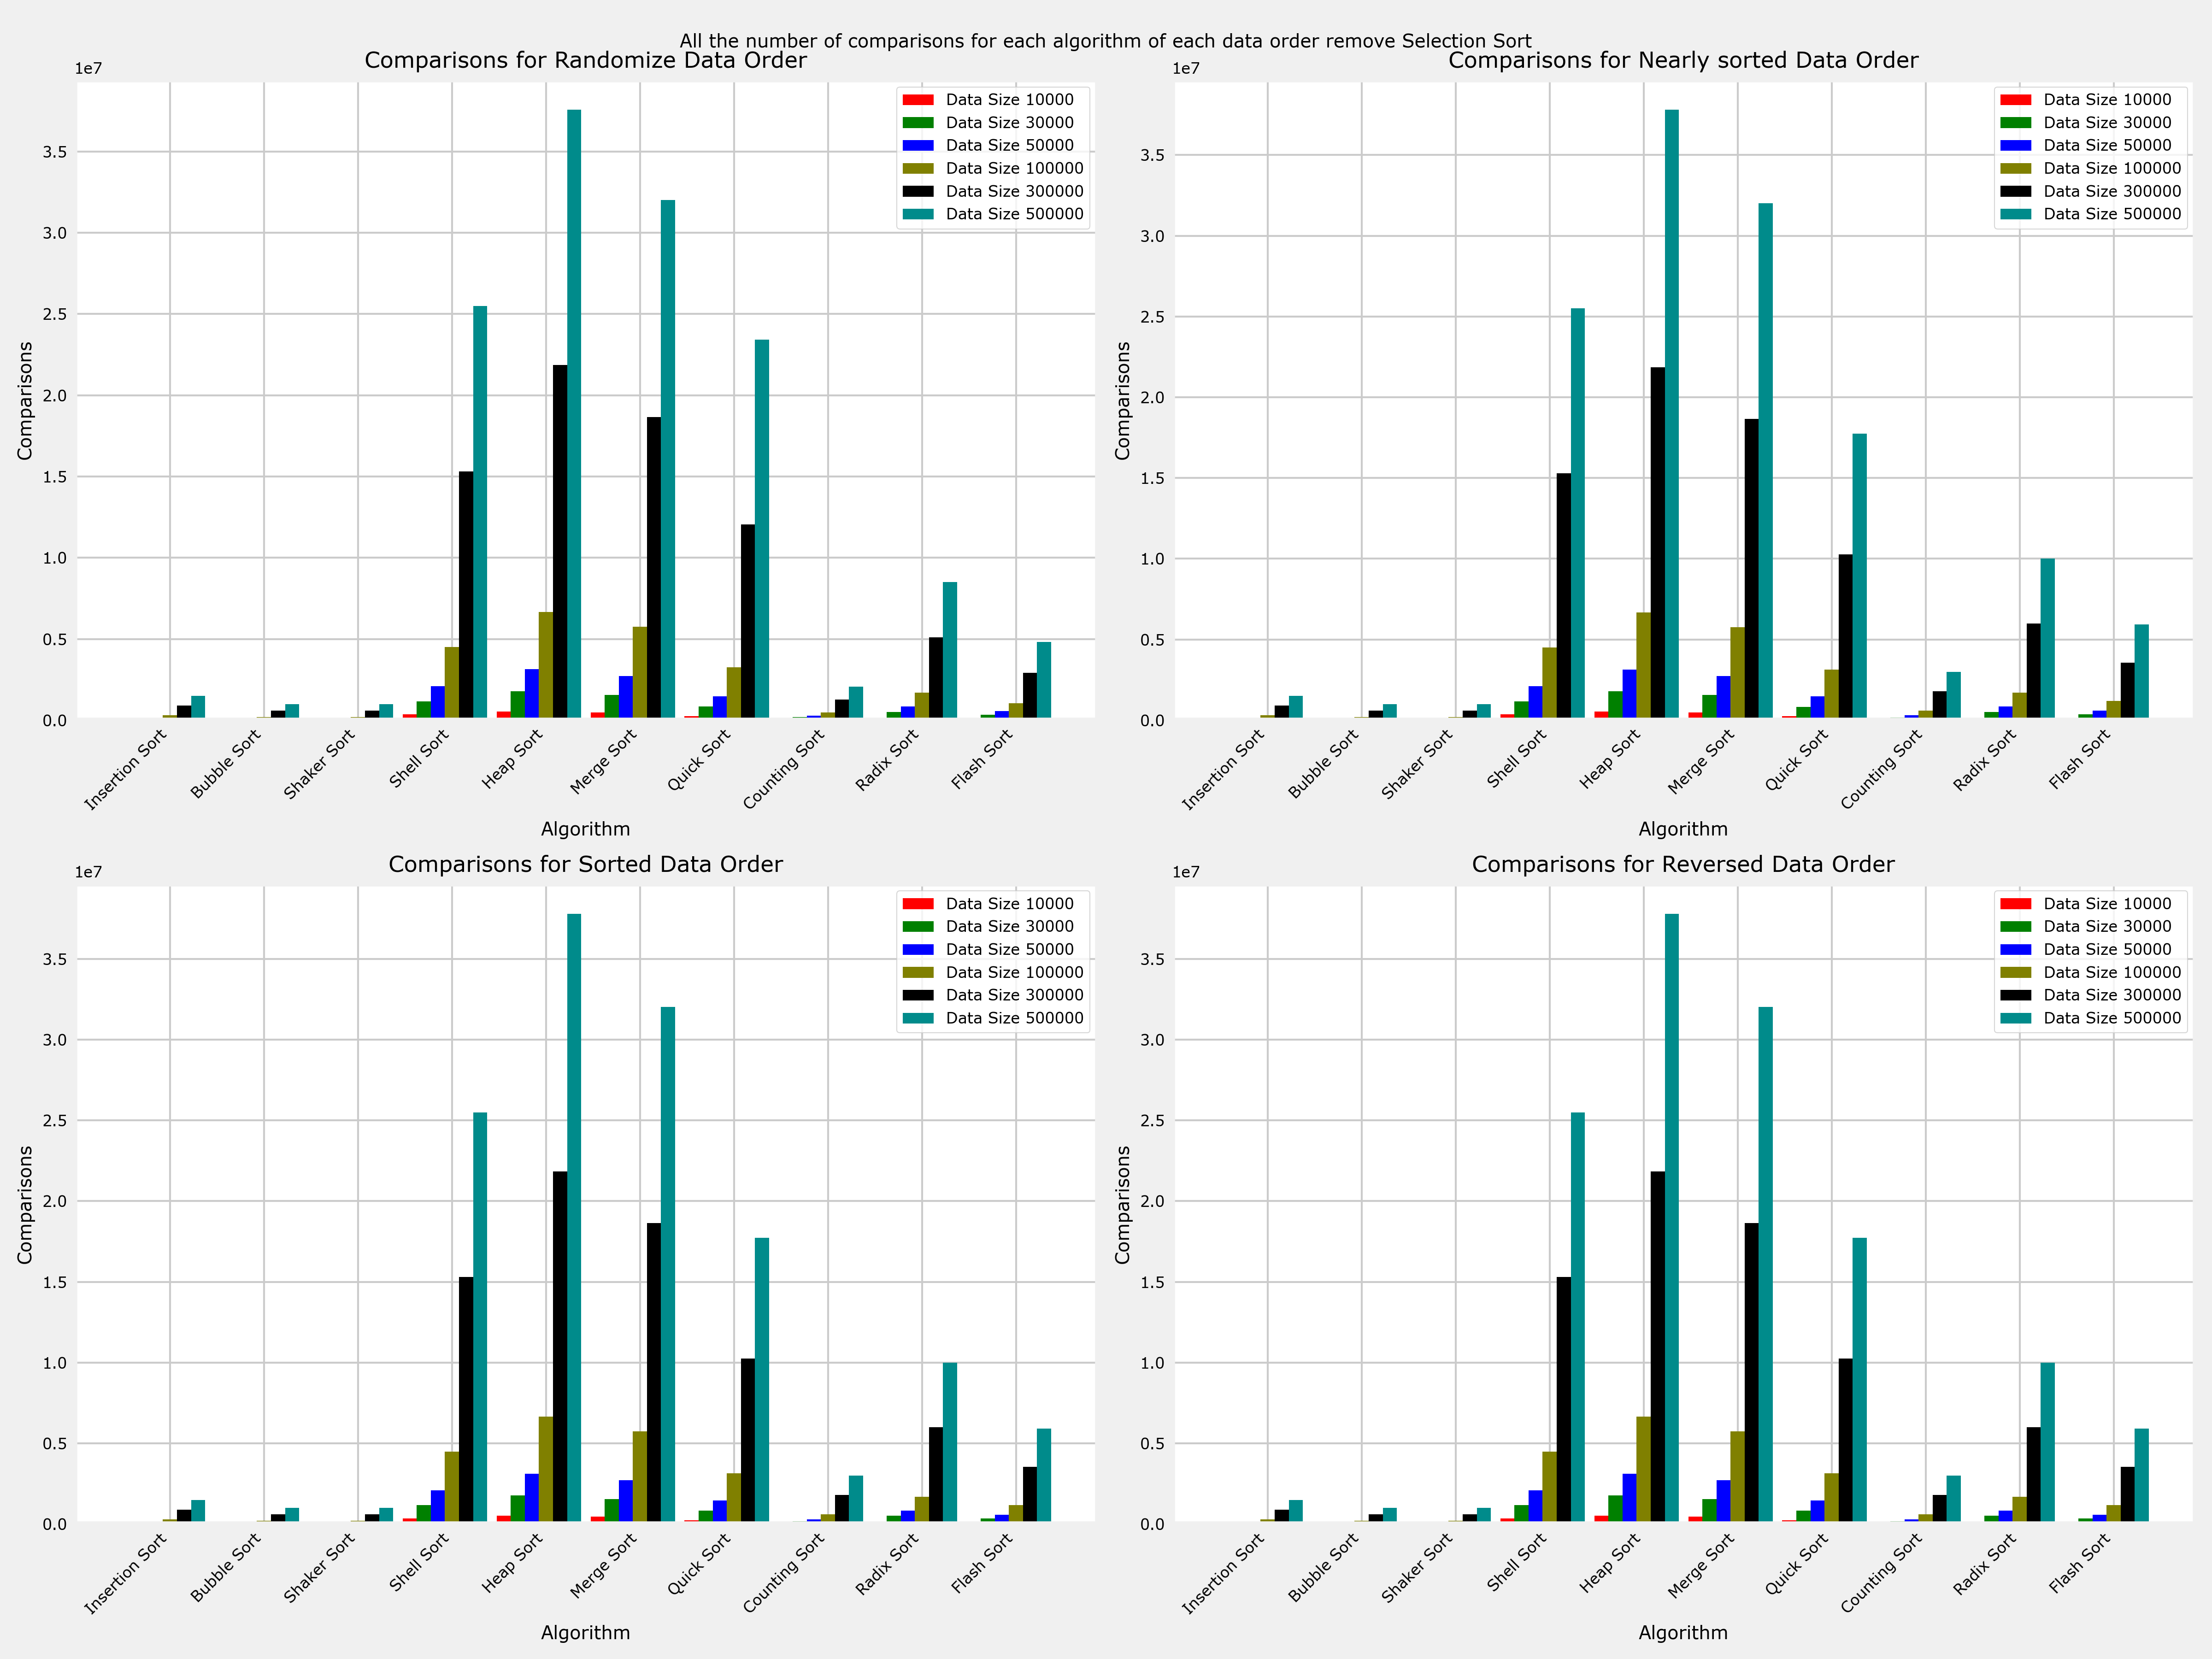
\includegraphics[width=\textwidth]{experimental_result/images/all_the_number_of_comparisons_for_each_algorithm_of_each_data_order_remove_selection_sort.png}
    \caption{Số phép so sánh của 10 thuật toán với tất cả trường hợp của dữ liệu (không có Selection Sort)}
    \label{fig:all_the_number_of_comparisons_for_each_algorithm_of_each_data_order_remove_selection_sort}
\end{figure}


Từ biểu đồ \ref{fig:all_the_number_of_comparisons_for_each_algorithm_of_each_data_order_remove_selection_sort} chia các thuật toán thành 3 nhóm chính: 
\begin{itemize}
    \item Nhóm 1: Insertion Sort, Bubble Sort, Shaker Sort 
    \item Nhóm 2: Shell Sort, Heap Sort, Merge Sort, Quick Sort
    \item Nhóm 3: Counting Sort, Radix Sort, Flash Sort
\end{itemize}

Nhóm 1 có số lượng phép so sánh ít nhất trong tất cả trường hợp của dữ liệu. Ngược lại, nhóm 2 lại có số phép sánh nhiều nhất trong ba nhóm.

Tiến hành nhìn kĩ hơn vào từng nhóm thuật toán.

\textbf{Nhóm 1}

\begin{figure}[H]
    \centering
    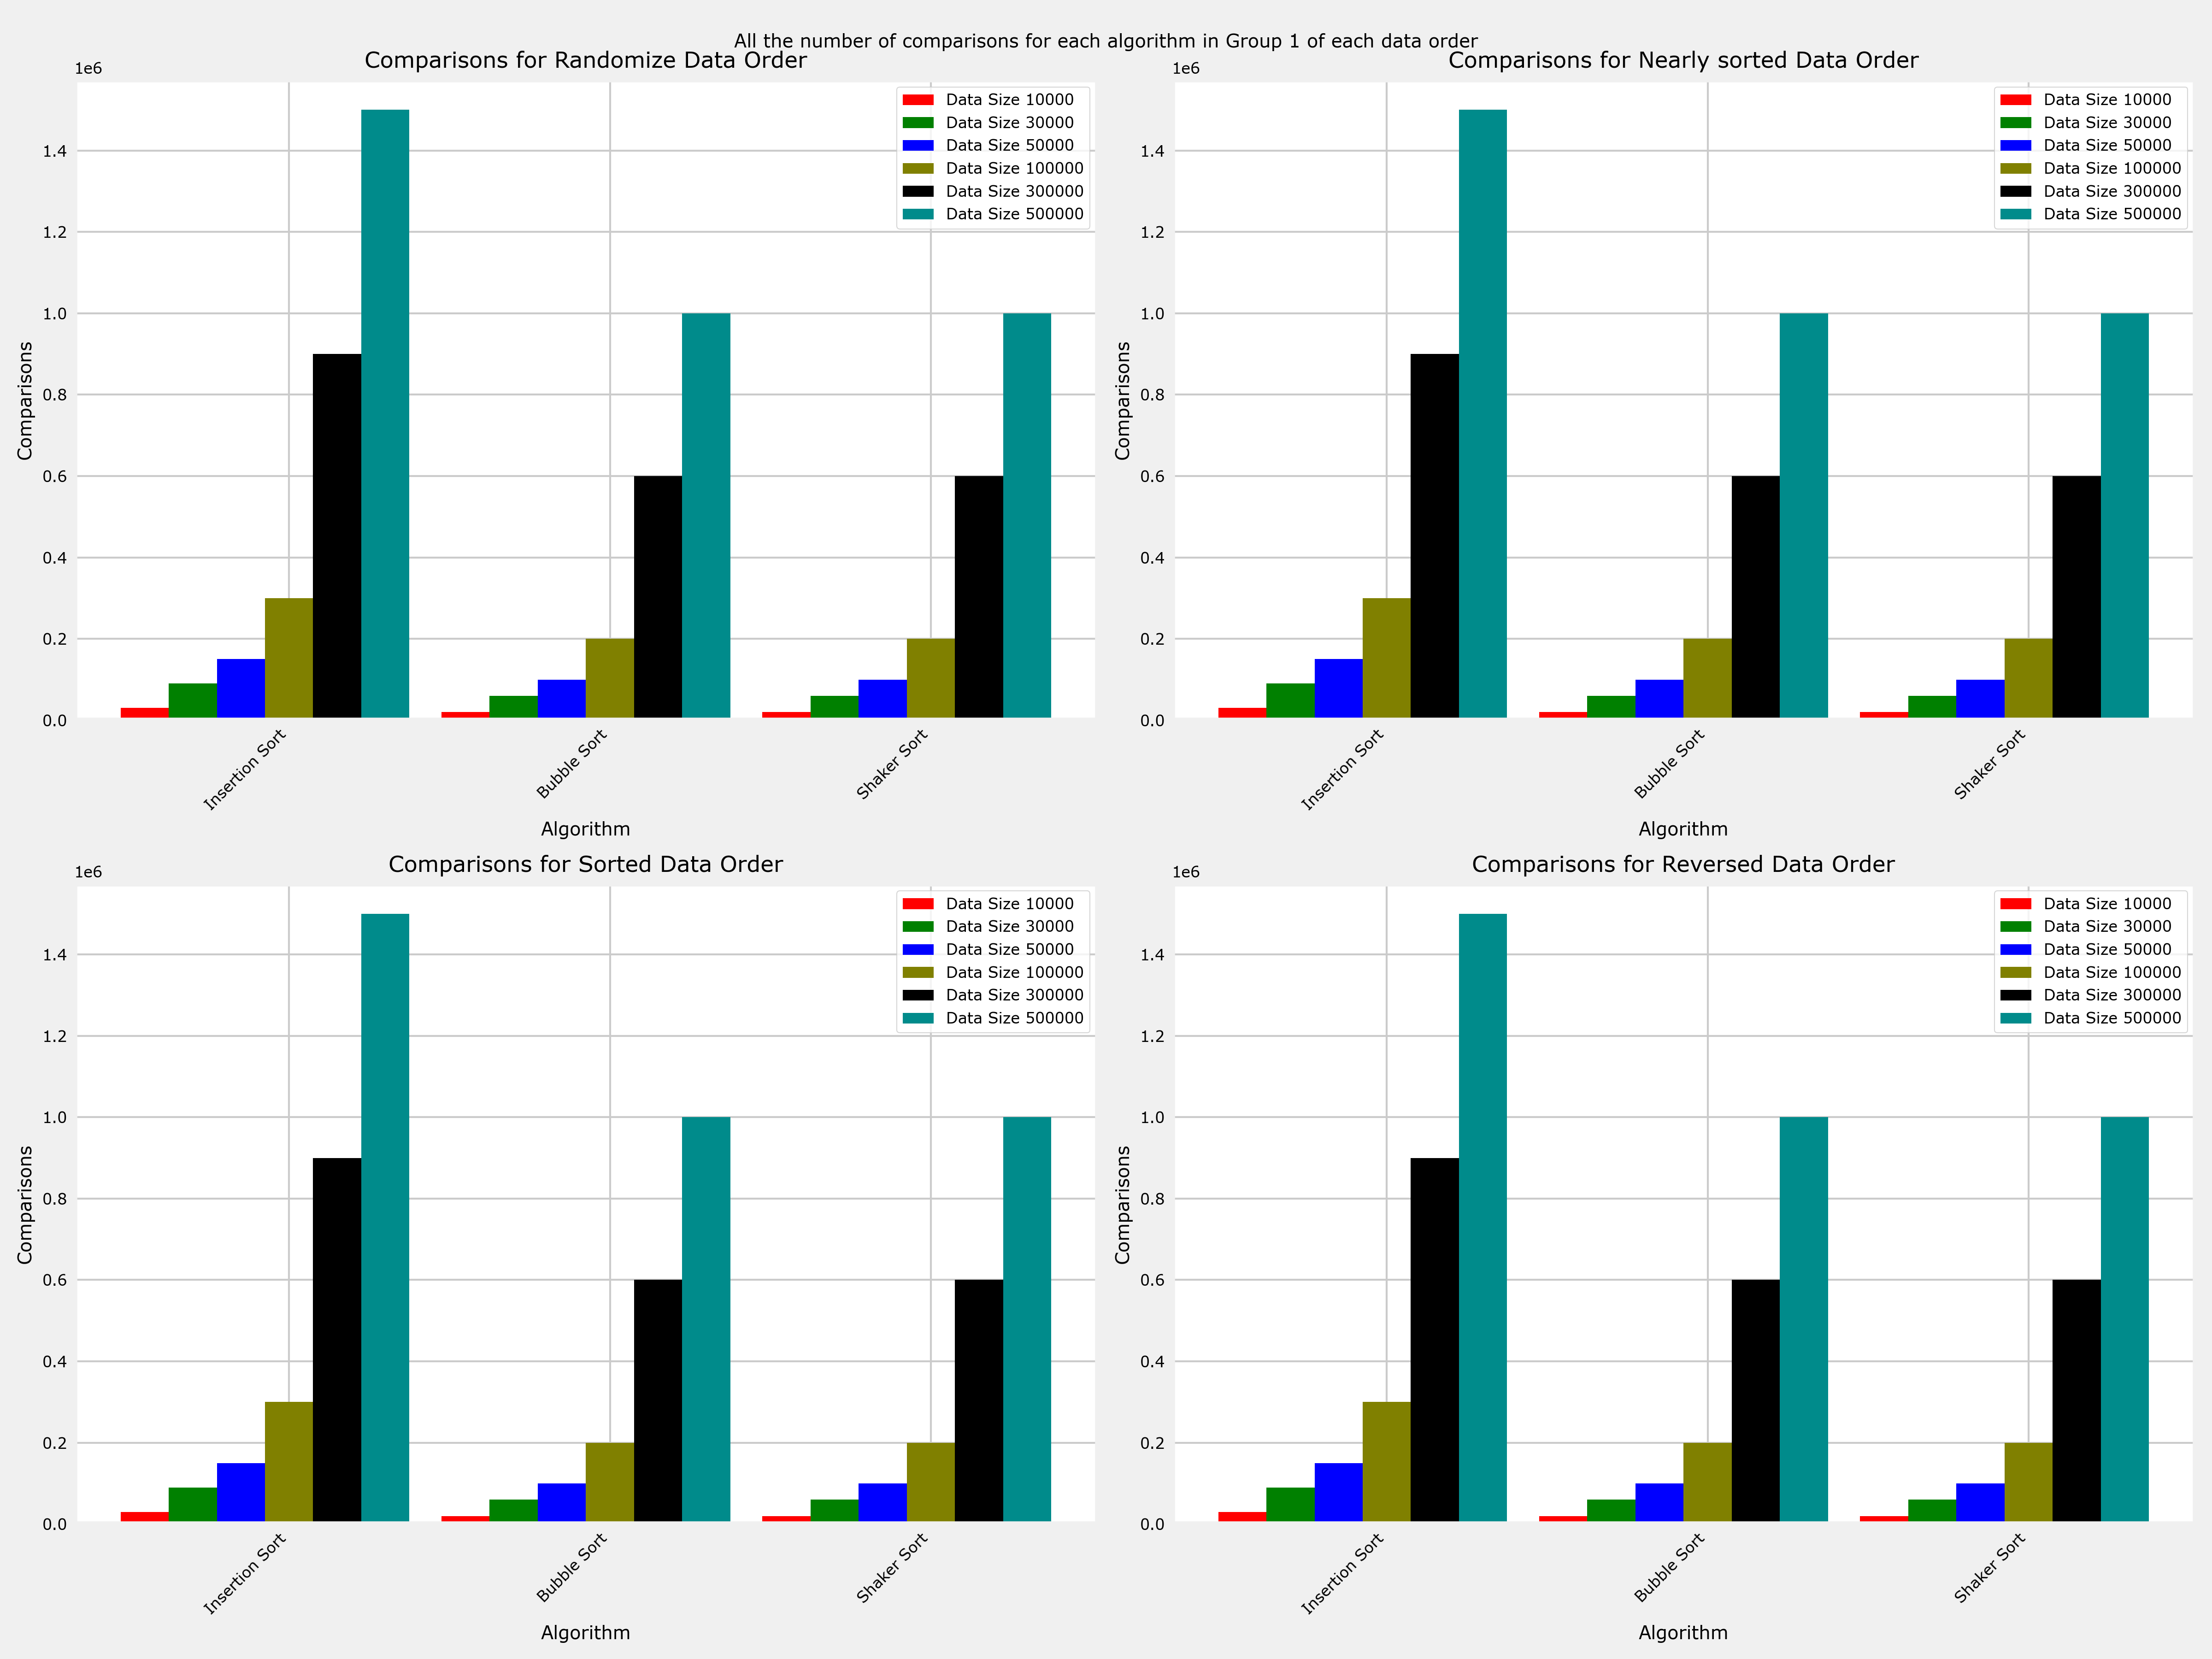
\includegraphics[width=\textwidth]{experimental_result/images/all_the_number_of_comparisons_for_each_algorithm_in_group_1_of_each_data_order.png}
    \caption{Số phép so sánh của Insertion Sort, Bubble Sort, Shaker Sort với tất cả trường hợp của dữ liệu}
    \label{fig:all_the_number_of_comparisons_for_each_algorithm_in_group_1_of_each_data_order}
\end{figure}

Ngoại trừ, Insertion Sort có độ phức tạp thời gian $\Theta(n)$ trong trường hợp mảng đã sắp xếp, các thuật toán nhóm này đều có xu hướng tăng theo hàm đa thức bậc hai. Điều này do các thuật toán này đều có độ phức tạp thời gian là hàm đa thức bậc hai cho trong hầu hết các trường hợp. 


\textbf{Nhóm 2}

\begin{figure}[H]
    \centering
    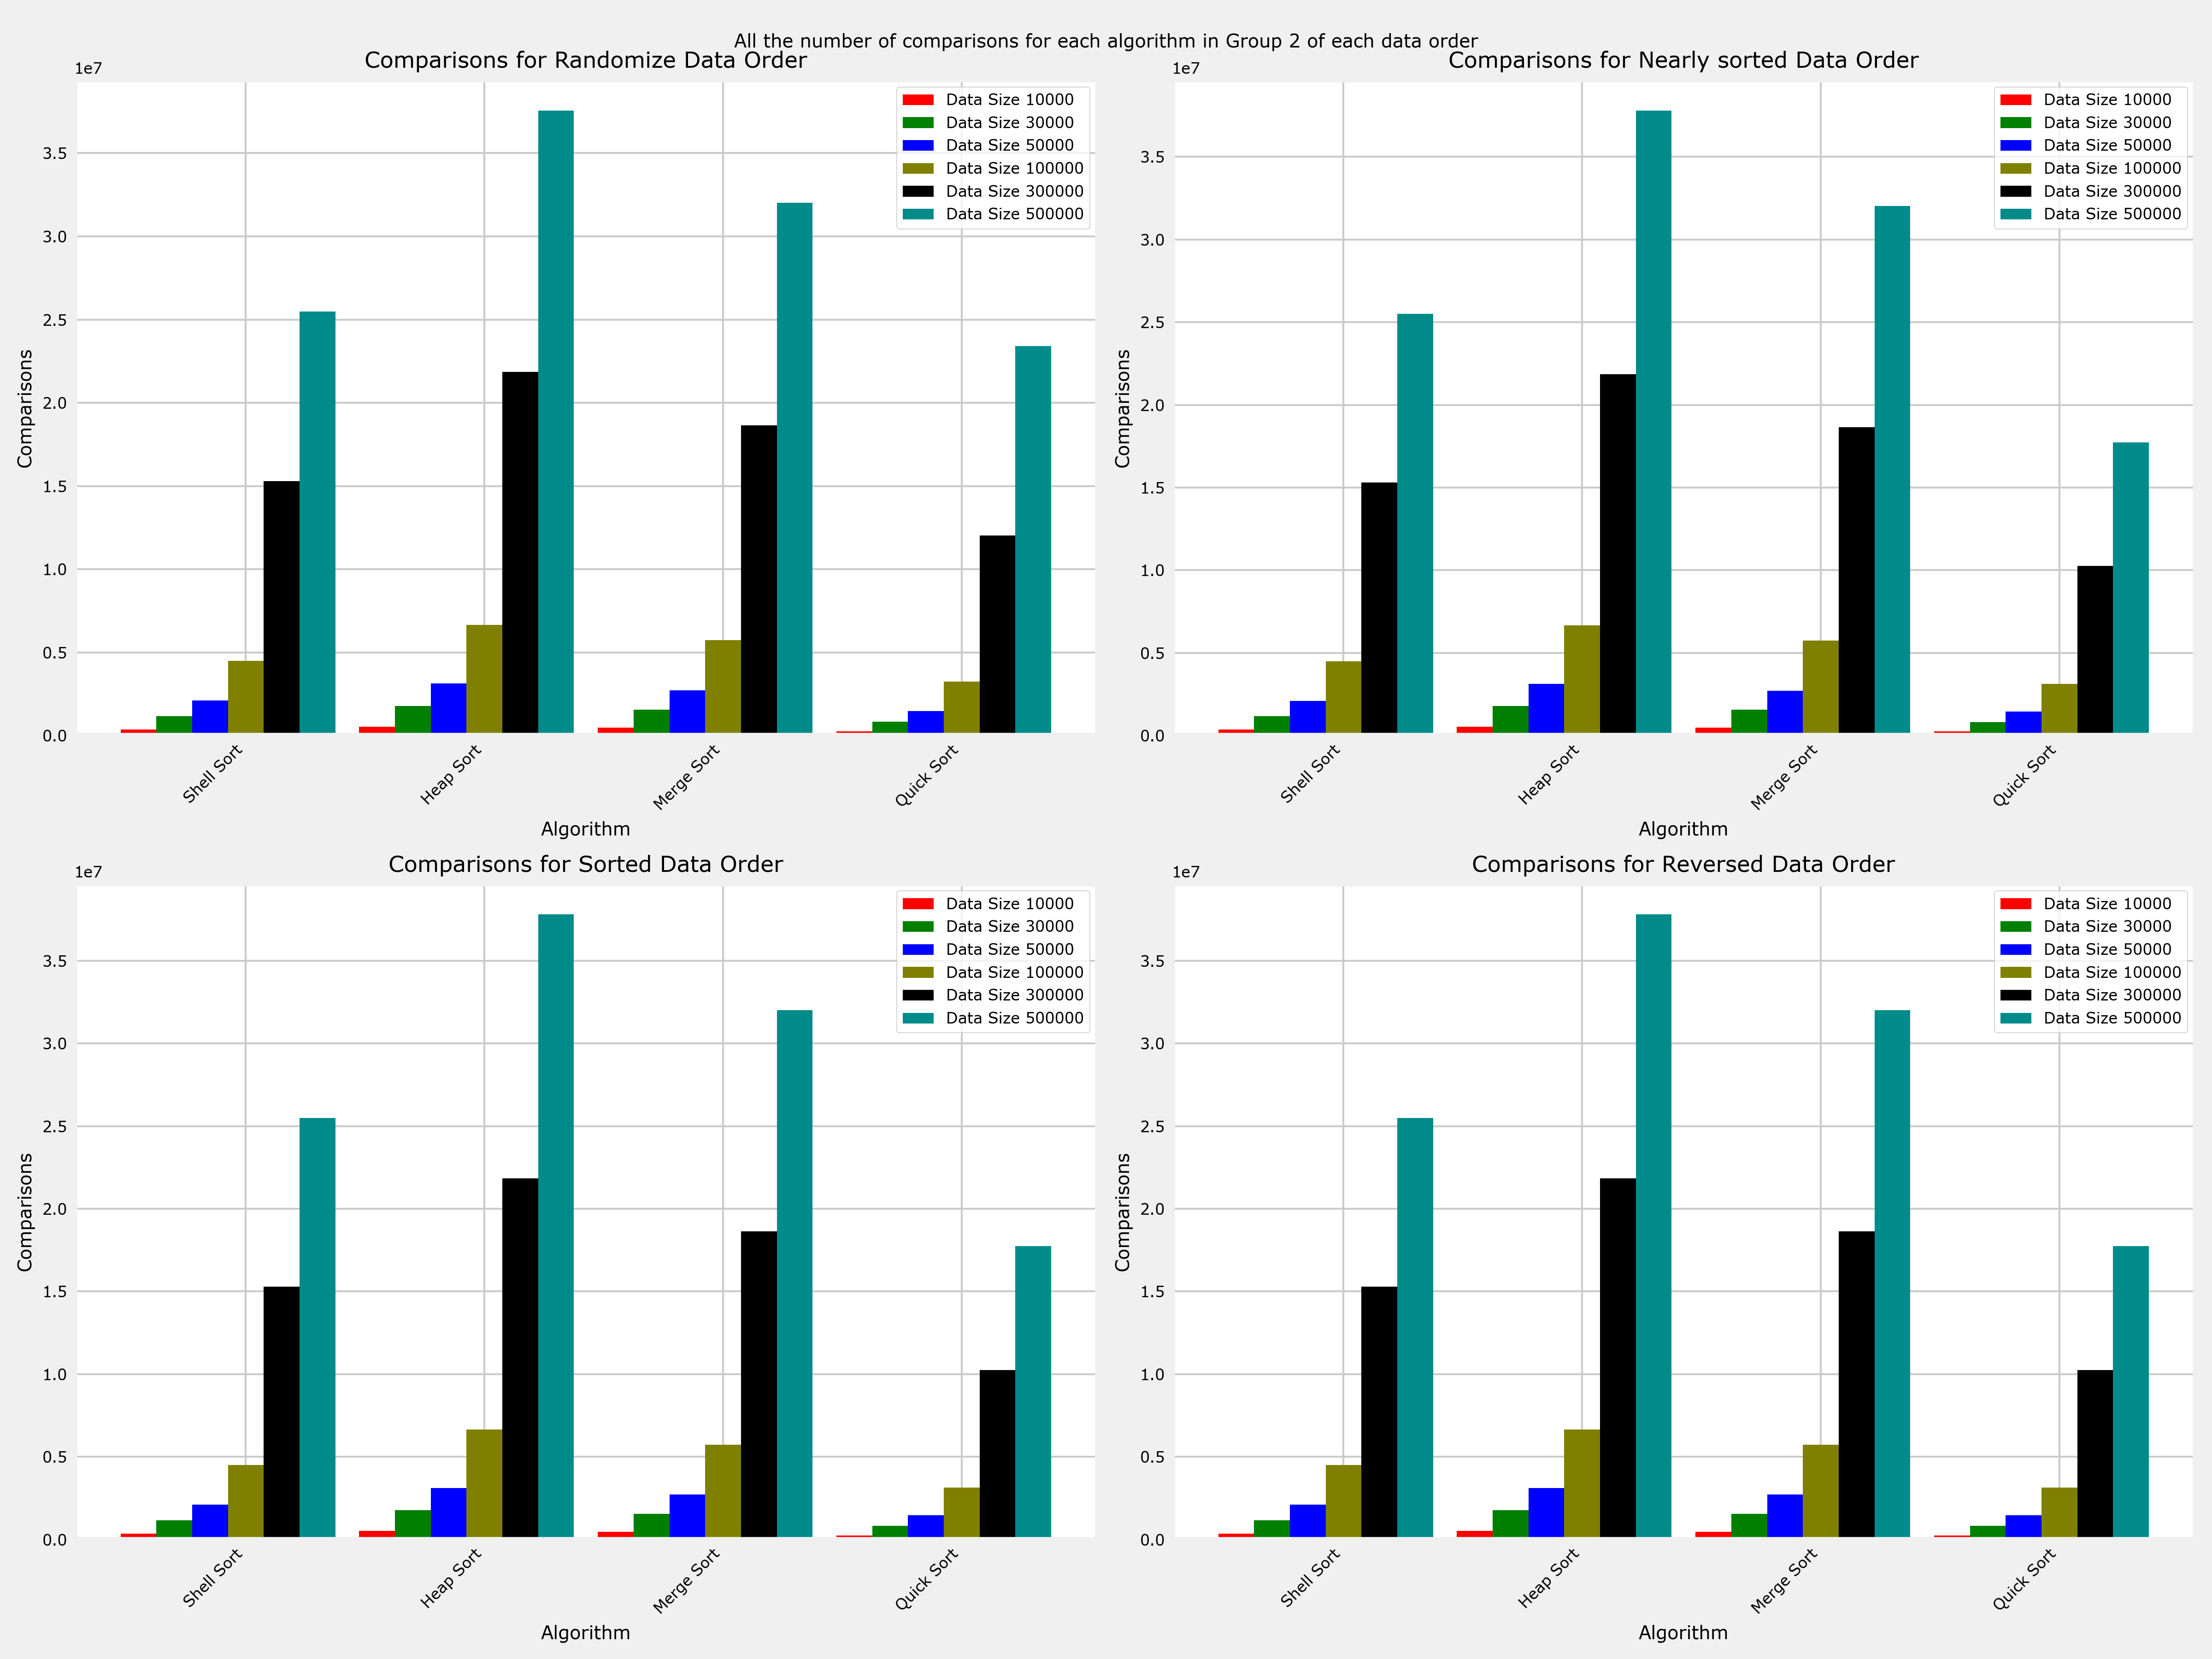
\includegraphics[width=\textwidth]{experimental_result/images/all_the_number_of_comparisons_for_each_algorithm_in_group_2_of_each_data_order.png}
    \caption{Số phép so sánh của Shell Sort, Heap Sort, Merge Sort, Quick Sort với tất cả trường hợp của dữ liệu}
    \label{fig:all_the_number_of_comparisons_for_each_algorithm_in_group_2_of_each_data_order}
\end{figure}

Đến với nhóm 2, số lượng phép so sánh của các thuật toán này không có hầu như không có sự thay đổi khi đi qua tất cả trường hợp của dữ liệu. Heap Sort có số lượng phép so sánh lớn nhất trong nhóm này, và thấp nhất là Quick Sort. 



\textbf{Nhóm 3}

\begin{figure}[H]
    \centering
    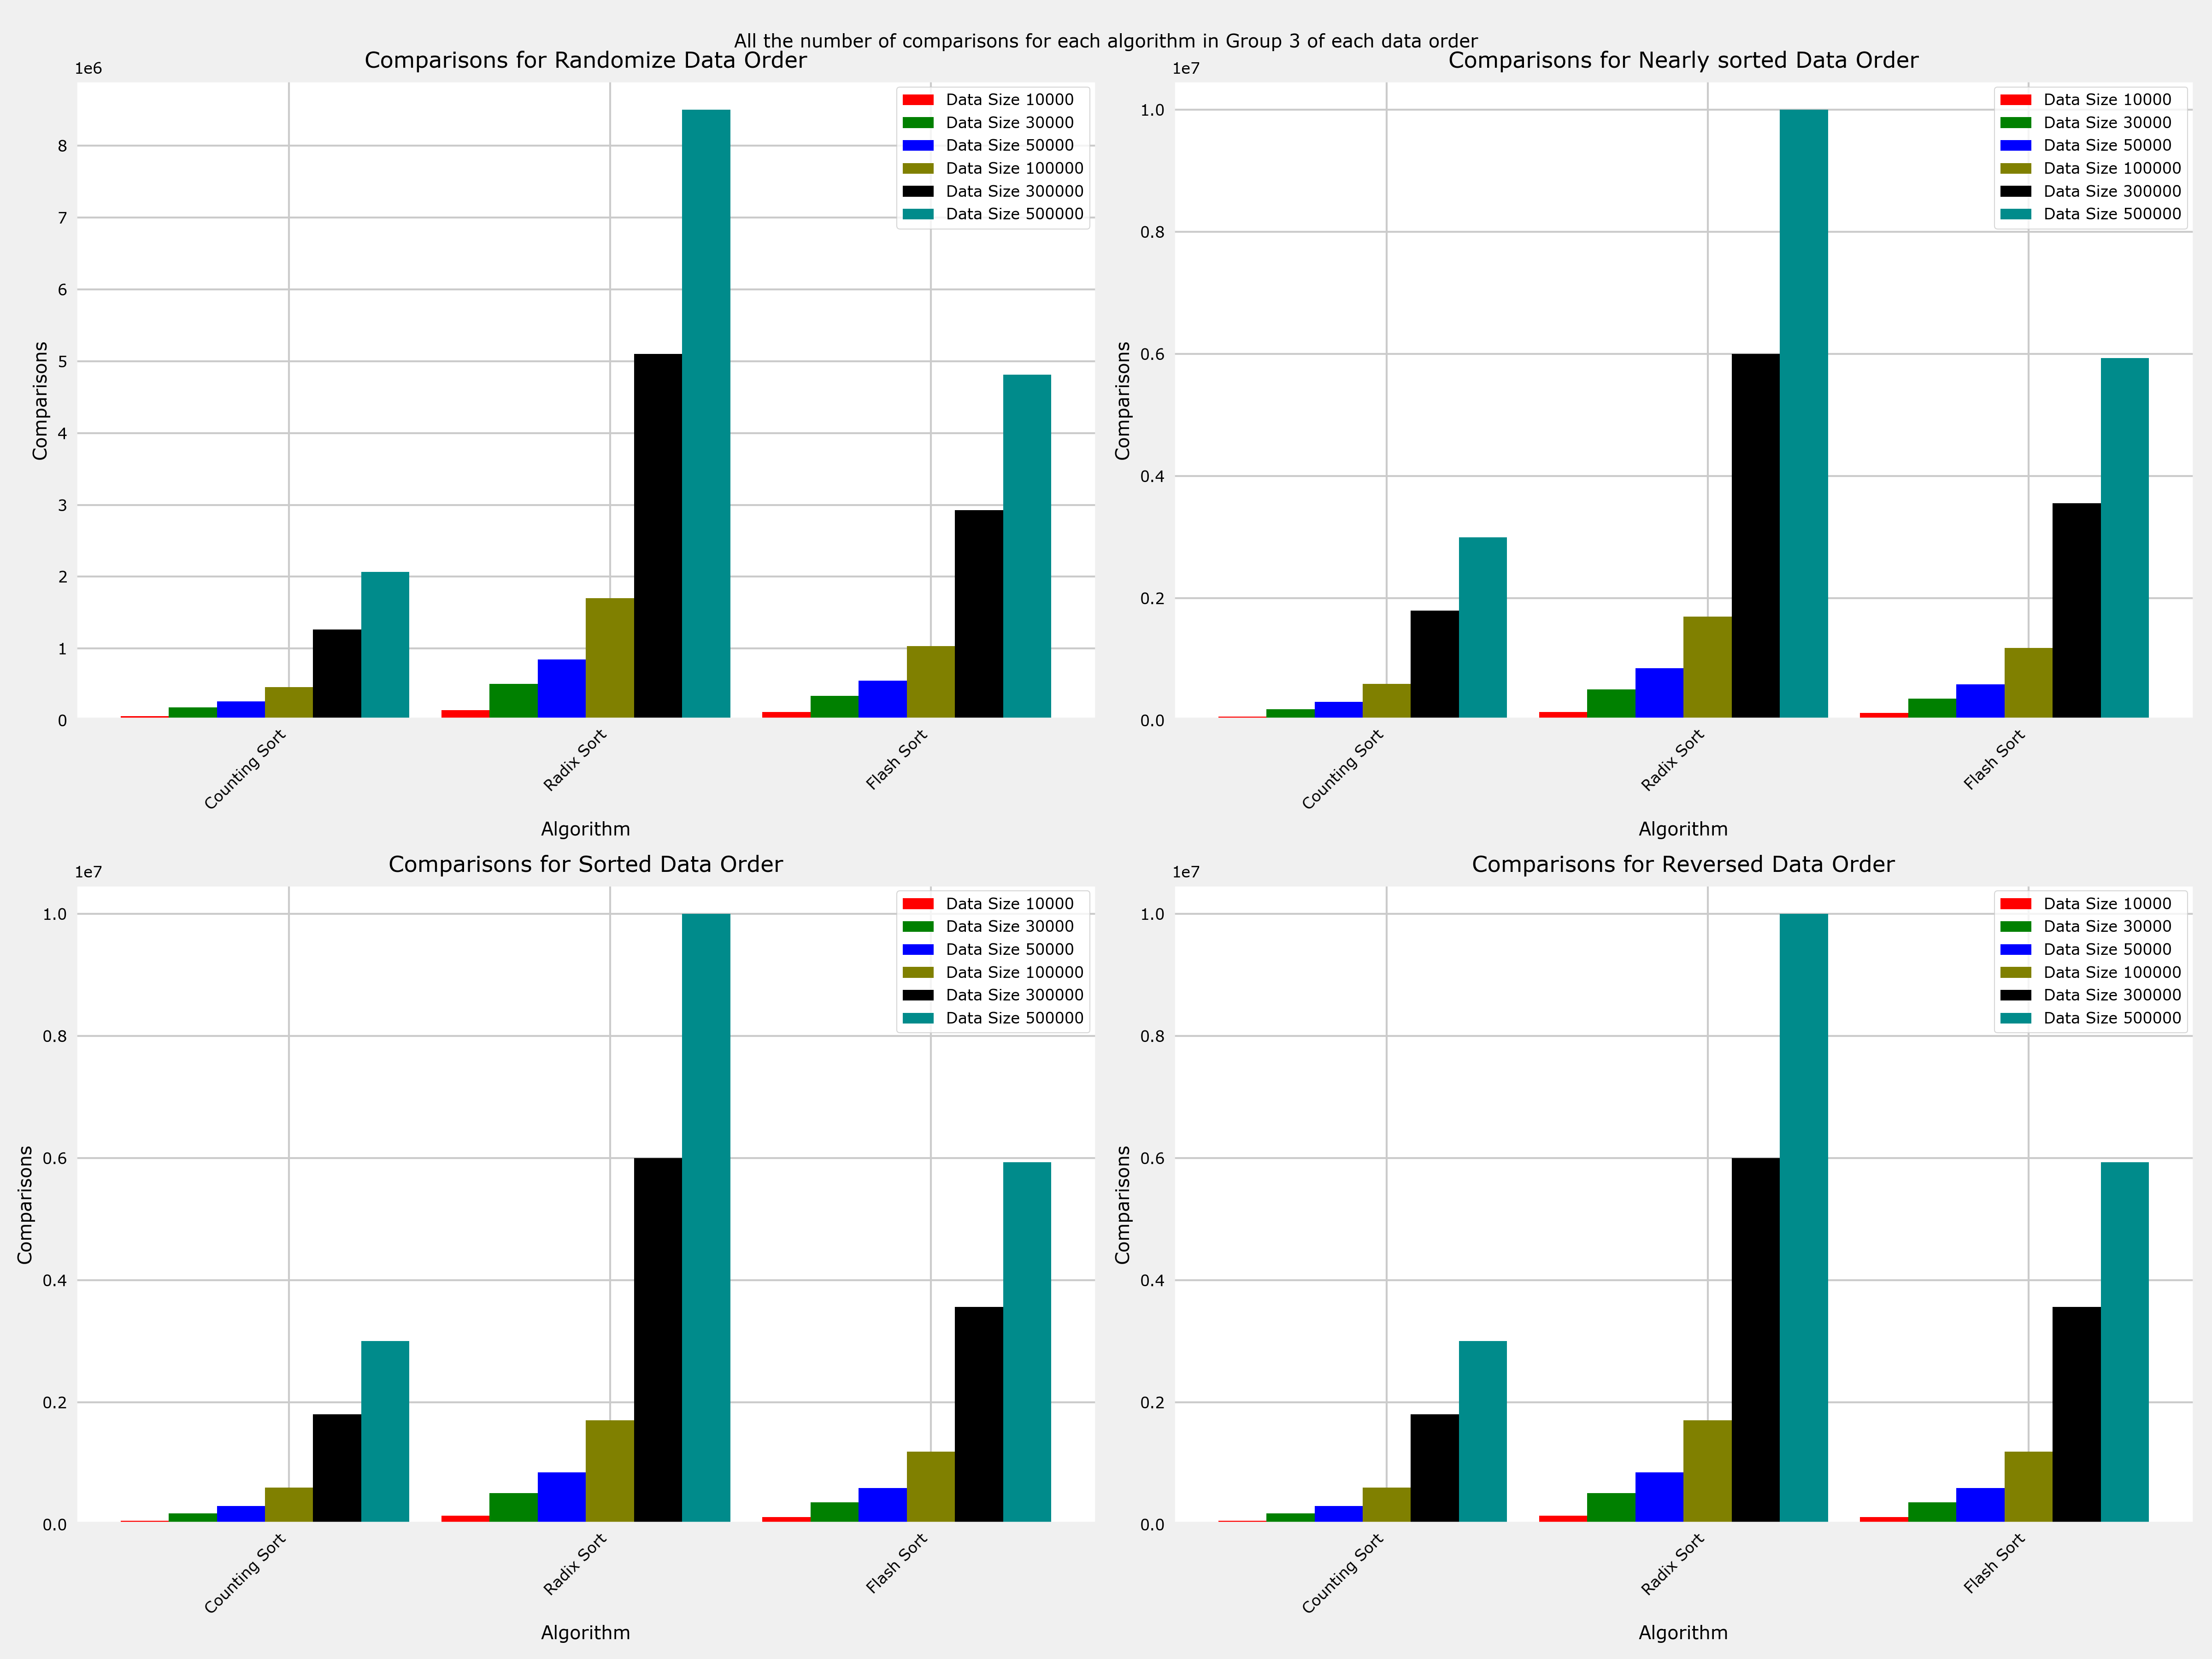
\includegraphics[width=\textwidth]{experimental_result/images/all_the_number_of_comparisons_for_each_algorithm_in_group_3_of_each_data_order.png}
    \caption{Số phép so sánh của Counting Sort, Radix Sort, Flash Sort với tất cả trường hợp của dữ liệu}
    \label{fig:all_the_number_of_comparisons_for_each_algorithm_in_group_3_of_each_data_order}
\end{figure}

Counting Sort thể hiển sự vượt trội của mình trong tất cả trường hợp, có độ tăng của số lượng phép so sánh khá thấp. Radix Sort có số phép so sánh nhiều nhất trong nhóm này. Flash Sort có số phép so sánh khá ổn định, có thể do sử dụng hàm \textbf{srand} để tạo ra dữ liệu chưa thật sự ngẫu nhiên.


\textbf{Nhận xét chung}

Các biểu đồ và hình ảnh trong phần kết quả thực nghiệm cho thấy sự khác biệt rõ rệt về hiệu suất của các thuật toán sắp xếp khi áp dụng trên các bộ dữ liệu khác nhau. 

\begin{itemize}
    \item Dữ liệu ngẫu nhiên: Các thuật toán cơ bản như Bubble Sort và Shaker Sort có thời gian chạy lớn hơn rất nhiều so với các thuật toán khác, thể hiện rõ độ phức tạp $O(n^2)$. Trong khi đó, các thuật toán như Counting Sort và Flash Sort có thời gian chạy rất nhỏ và ổn định.
    \item Dữ liệu gần sắp xếp hoàn chỉnh: Insertion Sort có thời gian thực thi nhanh nhất, phù hợp với trường hợp tốt nhất của nó. Các thuật toán cải tiến và không so sánh như Heap Sort, Radix Sort, Merge Sort vẫn giữ được tính ổn định.
    \item Dữ liệu được sắp xếp: Shaker Sort và Insertion Sort là hai thuật toán nhanh nhất, phù hợp với độ phức tạp thời gian $\Theta(n)$ trong trường hợp tốt nhất. Các thuật toán khác như Heap Sort, Radix Sort, Merge Sort vẫn giữ được tính ổn định.
    \item Dữ liệu đảo ngược: Shaker Sort có thời gian chạy chậm hơn Bubble Sort, trong khi Selection Sort và Insertion Sort có thời gian thực thi tương đối giống nhau. Các thuật toán như Heap Sort, Radix Sort, Merge Sort vẫn thể hiện được tính ổn định.
    \item Số phép so sánh: Selection Sort có số lượng phép so sánh vượt trội, đạt đến 2500049999 phép so sánh. Các thuật toán khác được chia thành ba nhóm chính: Nhóm 1 (Insertion Sort, Bubble Sort, Shaker Sort) có số lượng phép so sánh ít nhất, Nhóm 2 (Shell Sort, Heap Sort, Merge Sort, Quick Sort) có số phép so sánh nhiều nhất, và Nhóm 3 (Counting Sort, Radix Sort, Flash Sort) có số phép so sánh ổn định và thấp nhất.
    \item Các thuật toán nhóm cải tiến có 
\end{itemize}

Nhìn chung, các thuật toán cải tiến và không so sánh như Counting Sort, Flash Sort, Heap Sort, Radix Sort, Merge Sort thể hiện hiệu suất tốt và ổn định hơn so với các thuật toán cơ bản như Bubble Sort, Shaker Sort, và Selection Sort.